\livelloA{Simple regression}

\livelloB{Impurities in paints}

\begin{frame}
  \begin{description}
    \item[Data: ]paint.txt \\ 
    \item[Description: ]
      \begin{footnotesize}
        \begin{itemize}
          \item \textit{Stirrate}: identifies the rate of agitation (revolution) applied to the container (rpm, revolutions per minute);
          \item \textit{Impurity}: indentifies the number of impurities (lumps) present in the containers of paint.
        \end{itemize}
      \end{footnotesize}
    \item[Aims: ]
      \begin{footnotesize}
        The number of impurities (lumps) present in the containers of paint depends on the rate of agitation applied to the container. The aim is to determine the relation between the rate of agitation (revolution) and the number of lumps.
        \begin{itemize}
          \item[-] Let us compute the main descriptive statistics of \textit{Impurity}.
          \item[-] Let us compute the correlation between \textit{Impurity} and \textit{Stirrate}.
          \item[-] Let us graphically represent the relation between these variables.
          \item[-] Let us compute a simple linear regression between \textit{Stirrate} and \textit{Impurity}.
          \item[-] Does \textit{Stirrate} influence \textit{Impurity}? How?
          \item[-] How many variability is explained by the regression? Which is the residual variability?  
        \end{itemize}
      \end{footnotesize}
  \end{description}
\end{frame}

\begin{frame}
  Computation of descriptive statistics and B-W graphic of \textit{Impurity}:\\
  \vspace{.3cm}
  \begin{scriptsize}
    \begin{center}
      \begin{tabular}{|c|cccccc|c|}
        \hline
        \textbf{n} & \textbf{Min.} & \textbf{1st. Qu.} & \textbf{Median} & \textbf{Mean} & \textbf{3rd. Qu.} & \textbf{Max.} & \textbf{Sd}\\
        \hline
        12 & 8.40 & 11.45 & 14.00 & 13.87 & 16.42 & 18.90 & 3.4076\\
        \hline	
      \end{tabular}
    \end{center}
    \vspace{0.3cm}
    \begin{center}
      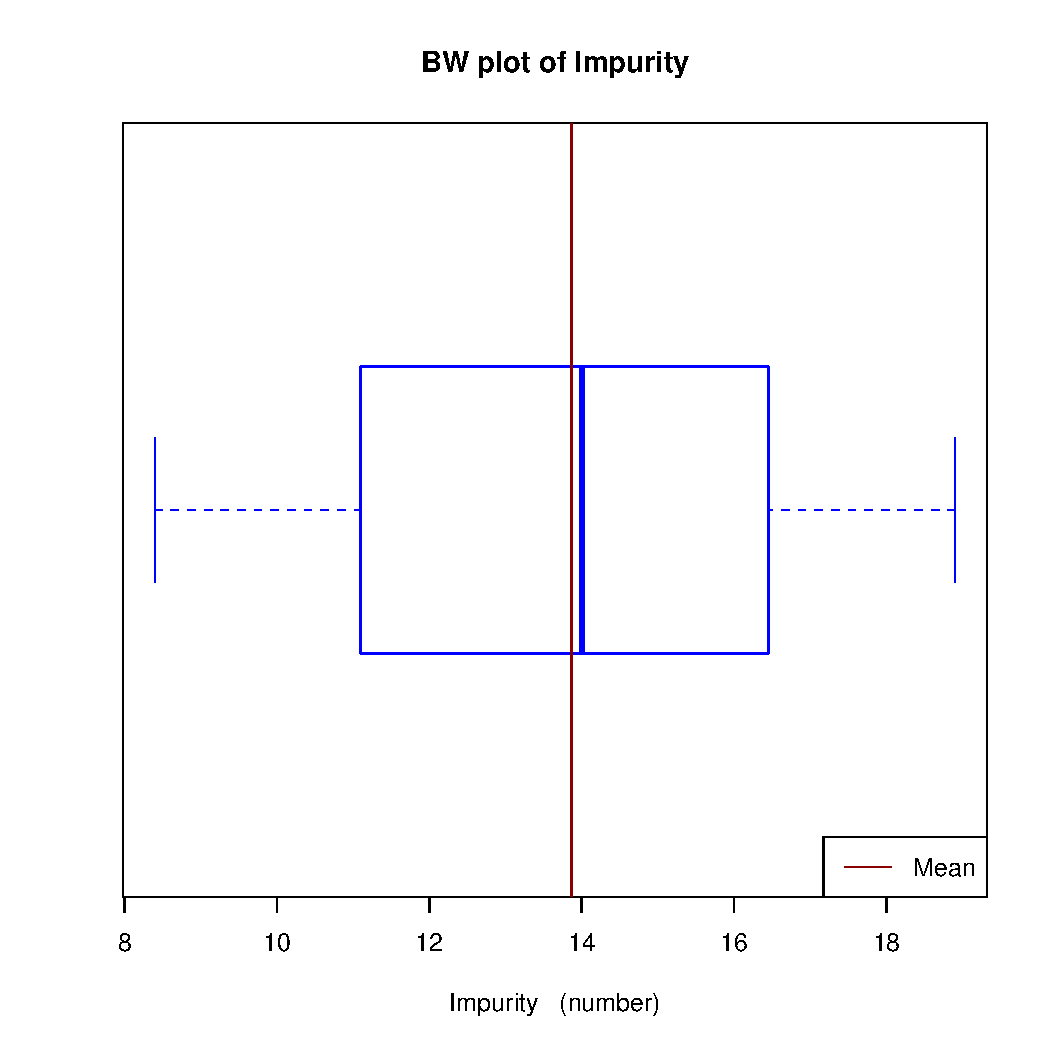
\includegraphics[width=6cm]{99_06_bwImpurity}
    \end{center}
  \end{scriptsize}
\end{frame}

\begin{frame}
  Scatterplot matrix of the relation between correlation and significativity: \\
  \begin{center}
    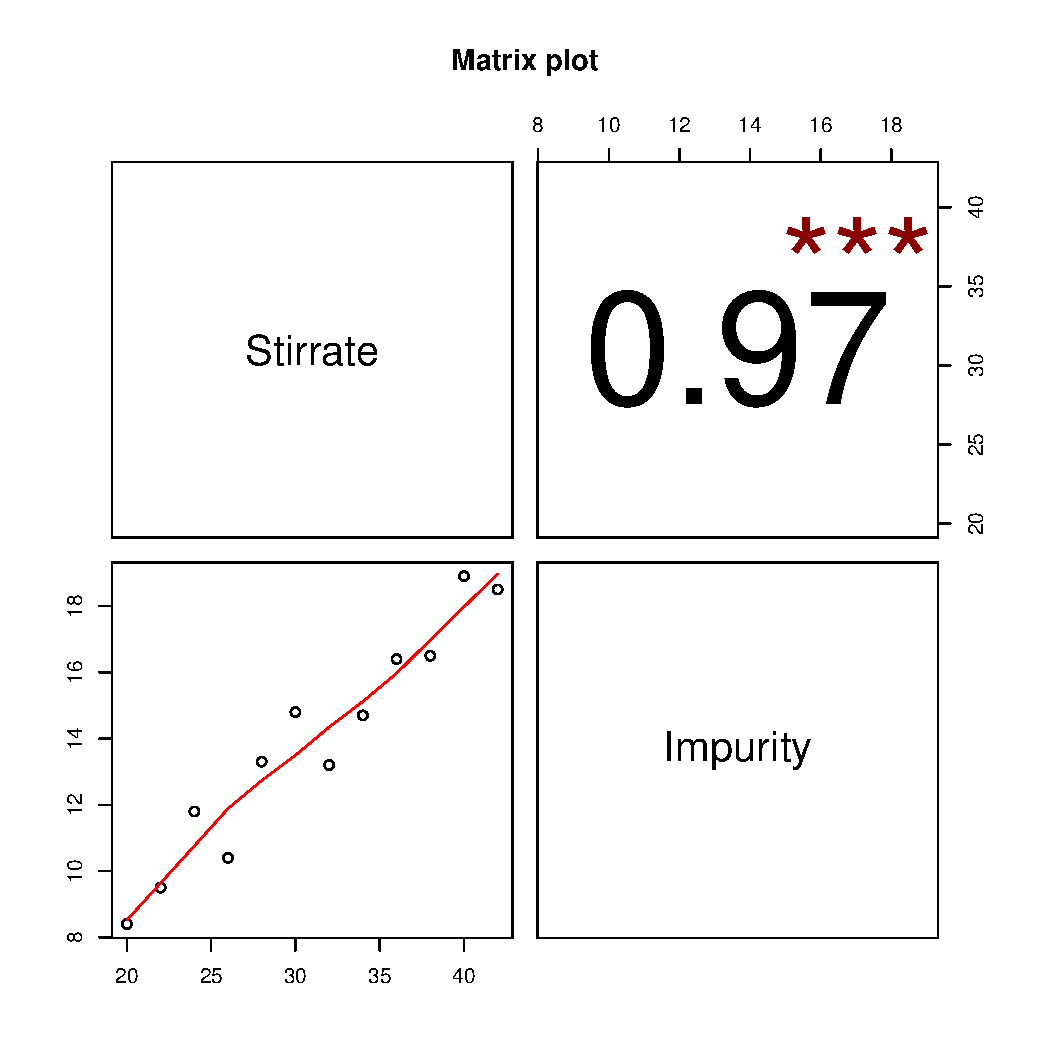
\includegraphics[width=5.5cm]{99_06_splmatImpurity}
  \end{center}
\end{frame}

\begin{frame}
  Scatterplot of the relation with the regression line:\\
  \vspace{.3cm}
  \begin{center}
    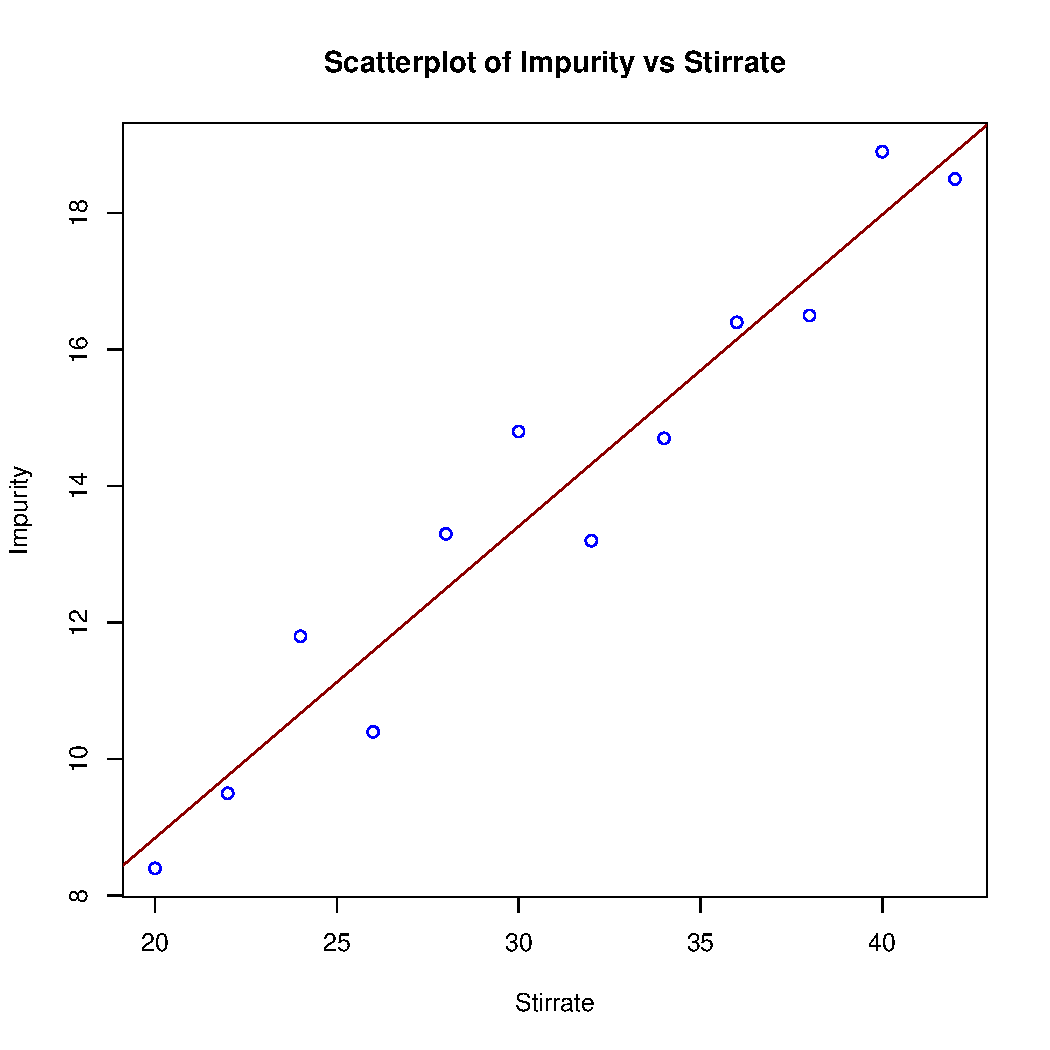
\includegraphics[width=7.5cm]{99_06_regrStirrateImpurity}
  \end{center}
\end{frame}

\begin{frame}[fragile]
  Regression analysis:\\
  \begin{small}
    \begin{verbatim}
Coefficients:
               Estimate  Std. Error  t value   p value    
(Intercept)    -0.28928     1.22079   -0.237     0.817
Stirrate        0.45664     0.03844   11.880  3.21e-07

Residual standard error: 0.9193 on 10 degrees of freedom
Multiple R-squared: 0.9338,	Adjusted R-squared: 0.9272 
F-statistic: 141.1 on 1 and 10 DF,  p-value: 3.211e-07
    \end{verbatim}
  \end{small}
  Anderson-Darling test:\\
  \begin{small}
    \begin{verbatim}
A = 0.4329, p-value = 0.2515
    \end{verbatim}
  \end{small}
\end{frame}

\begin{frame}
  Graphical check of the regression model:\\
  \vspace{.1cm}
  \begin{center}
    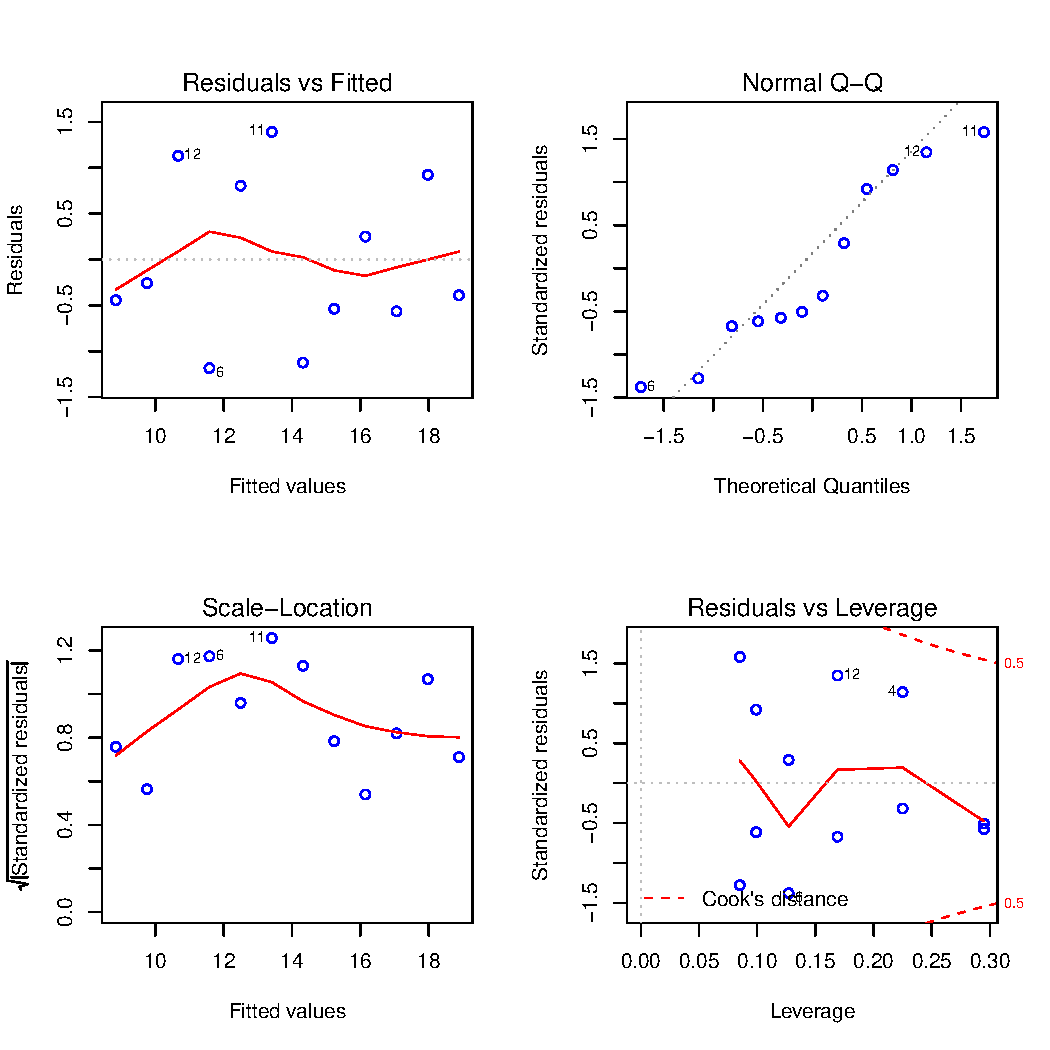
\includegraphics[width=7.5cm]{99_06_residStirrateImpurity}
    \end{center}
\end{frame}

\begin{frame}
  \begin{small}
    \begin{itemize}
      \item The relation that ``links'' the revolution rate seems to be well described by a simple linea regression, at least for the considered interval of \textit{Stirrate}.  
      \item The estimated formula is the follows: $ Impurity = -0.2893 + 0.4566 \cdot Stirrate $.
      \item The p-value for the significativity of the coefficient of \textit{Stirrate} is extremely low. This fact confirms the ``non random'' existing relation between the two variables.  
      \item $ R^2 $ value is equal to 0.9338; this fact confirms that the model explais well the observed data.
      \item The standard deviation of the residual is 0.9193.
      \item The p-value of the intercept estimate is 0.817. This would indicate an intercept potentially equal to 0. 
      \item Keeping the intercept value equal to the estimate,  with value of \textit{Stirrate}=0, the mean number of imputities would be negative: the results of the regression couldn't be ``extended'' too outside experimental field. 
    \end{itemize}
  \end{small}
\end{frame}

\livelloB{Resistance of a polypropylene film}

\begin{frame}
  \begin{description}
    \item[Data: ]temperatures.txt \\ 
    %\item[Origine dati: ]http://www.weibull.com/DOEWeb/simple_linear_regression_analysis.htm\\
    \item[Description: ]
      \begin{footnotesize}
        \begin{itemize}
          \item \textit{Yield}: indicates the resistance of a polypropylene film;
          \item \textit{Temperature}: indicates the temperature of a chemical process.
        \end{itemize}
      \end{footnotesize}
    \item[Aims: ]
      \begin{footnotesize}
        The resistance of a polypropylene film depends on the temperature on which the chemical process is performed. The aim is to determine the relation between resistance and temperature.
        \begin{itemize}
          \item[-] Let us graphically represent the relation between the two variables.
          \item[-] Let us compute a simple linear regression between \textit{Yield} and \textit{Temperature}.
          \item[-] Does \textit{Yield} influences \textit{Temperature}? How?
          \item[-] How many variability is explained by the regression? Which is the residual variability?    
        \end{itemize}
      \end{footnotesize}
  \end{description}
\end{frame}

\begin{frame}
%   \begin{small}
    \begin{itemize}
      \item The relation  that ``links'' the revolution rate with the number of impurities seems to be well described by a simple linear regression, at least in the considered interval of \textit{Stirrate}. 
      \item The estimated formula is the follows: $ Yield = 17.00 + 2.00 \cdot Temperature $.
      \item The p-value for the significativity of the coefficient of \textit{Temperature} is extremely low. This fact confirms the ``non random'' existing relation between the two variables.
      \item $ R^2 $ value is 0.9831. This fact confirms that the model explains well the observed data.
    \end{itemize}
%   \end{small}
\end{frame}

\begin{frame}
  \begin{description}
    \item[Data: ]production.txt \\ 
    %\item[Origine dati: ]http://www.stat.tamu.edu/~sheather/book/docs/datasets/production.txt\\
    \item[Description: ]
      \begin{footnotesize}
        \begin{itemize}
          \item \textit{RunSize}: indicates the number of pieces produced in a productive process;
          \item \textit{RunTime}: indicates the duration of a productive process.
        \end{itemize}
      \end{footnotesize}
    \item[Aims: ]
      \begin{footnotesize}
        The duration of a productive process depends on the number of pieces produced.
        \begin{itemize}
          \item[-] Let us graphically represent the relation between the two variables.
          \item[-] Let us compute a simple linear regression between \textit{RunTime} a \textit{RunSize}.
          \item[-] Does \textit{RunSize} influences \textit{RunTime}? How?
          \item[-] How many variability is explained by the regression? Which is the residual variability? 
        \end{itemize}
      \end{footnotesize}
  \end{description}
\end{frame}

\begin{frame}
%   \begin{small}
    \begin{itemize}
      \item The relation that ``links'' the duration of the productiove process with the number of pieces produced seems to be well descibed by a simple linear regression.
      \item The esimated formula is the follows:  $ RunTime = 149.75 + 0.26 \cdot RunSize $.
      \item The p-value for the significativity of the coefficient of \textit{RunSize} is extremely low. This fact confirms the ``non random'' existing relation between the two variables.
      \item $ R^2 $ value is 0.7302. This fact confirms that the model explains well the observed data.
    \end{itemize}
%   \end{small}
\end{frame}


\livelloA{Polynomial regression}

\livelloB{Pressure Switch}

\begin{frame}
  \begin{description}
    \item[Data: ]switch.txt \\ 
    \item[Description: ]
      \begin{footnotesize}
        \begin{itemize}
	  \item \textit{BuildOrder}: indicates the order in which the switches have been assembled;
          \item \textit{RunOrder}: indicates the order in which the observations have been collected;
          \item \textit{DThickness}: indicates the thickness of the diaphragm (mm);
          \item \textit{SetPoint}: indicates the pressure at which the switch opens (KPa).
        \end{itemize}
      \end{footnotesize}
    \item[Aims: ]
      \begin{footnotesize}
        A pressure switch has a membrane whose thickness (in mm) influences the pressure required to trigger the switch itself. The aim is to determine the thickness of the membrane for which the switch ``trig'' with a pressure equal to $165 \pm 15$ KPa. 25 switches with different thickness of the membrane was analysed. 
        \begin{itemize}
          \item[-] Let us compute the descriptive statistics of the variable \textit{SetPoint}.
          \item[-] Let us graphically represent the relation \textit{DThickness}-\textit{SetPoint}.
          \item[-] Let us compute a linear regression between the two variables.
          \item[-] Does \textit{DThickness} influences \textit{SetPoint}? Is the model correct?
          %\item[-] Si determini lo spessore della membrana per cui l'interruttore ``scatta'' con una pressione pari a $165 \pm 15$ KPa.
          \item[-] How can be modified the model? Which are the final characteristics?
        \end{itemize}
      \end{footnotesize}
  \end{description}
\end{frame}

\begin{frame}
  Computation of the descriptive statistics and of the B-W Graphic of \textit{SetPoint}:\\
  \vspace{.3cm}
  \begin{scriptsize}
    \begin{center}
      \begin{tabular}{|c|cccccc|c|}
        \hline
        \textbf{n} & \textbf{Min.} & \textbf{1st. Qu.} & \textbf{Median} & \textbf{Mean} & \textbf{3rd. Qu.} & \textbf{Max.} & \textbf{Sd}\\
        \hline
        25 & 144.7 & 157.4 & 174.8 & 181.1 & 200.0 & 231.7 & 27.70 \\
        \hline	
      \end{tabular}
    \end{center}
    \vspace{0.3cm}
    \begin{center}
      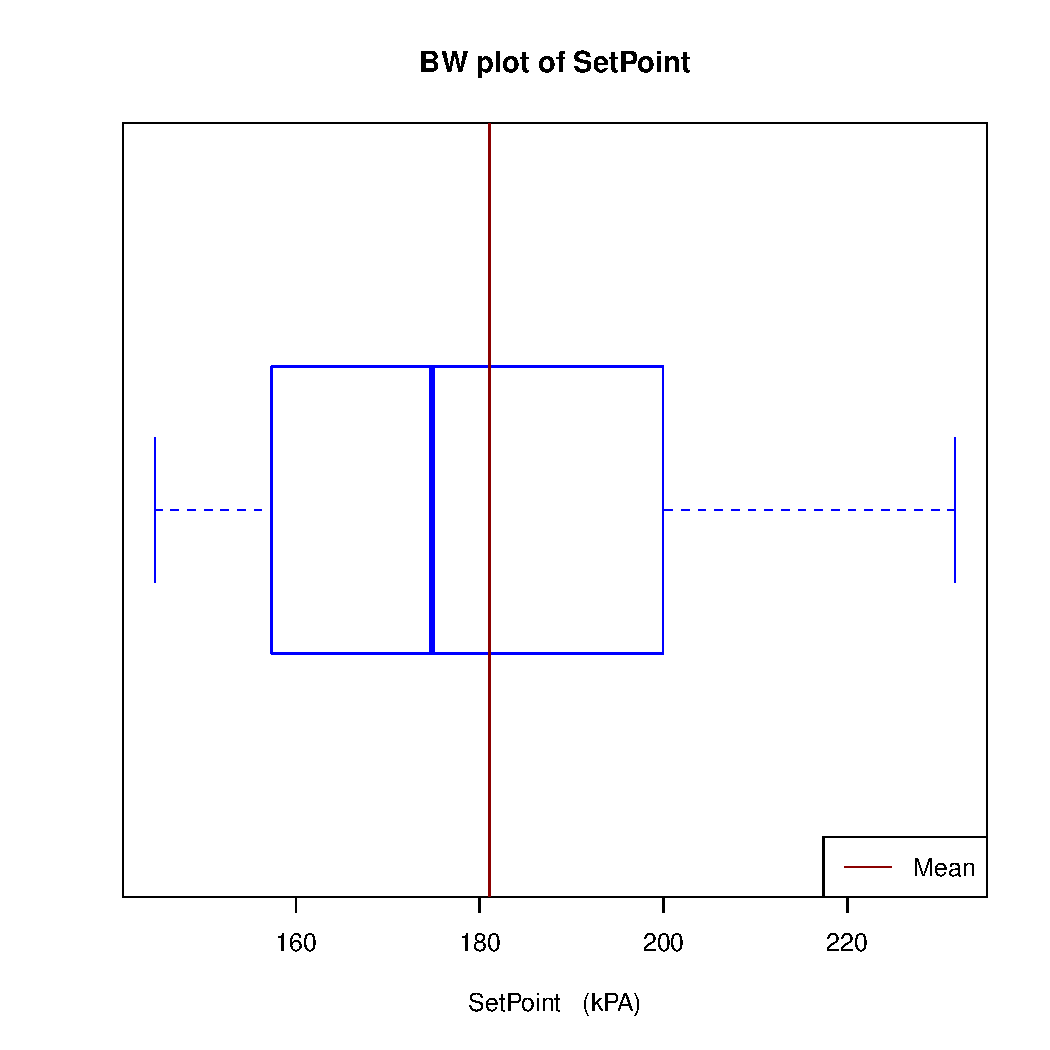
\includegraphics[width=6cm]{99_06_bwSetPoint}
    \end{center}
  \end{scriptsize}
\end{frame}

\begin{frame}
  Scatterplot of the relation with regression line:\\
  \vspace{.3cm}
  \begin{center}
    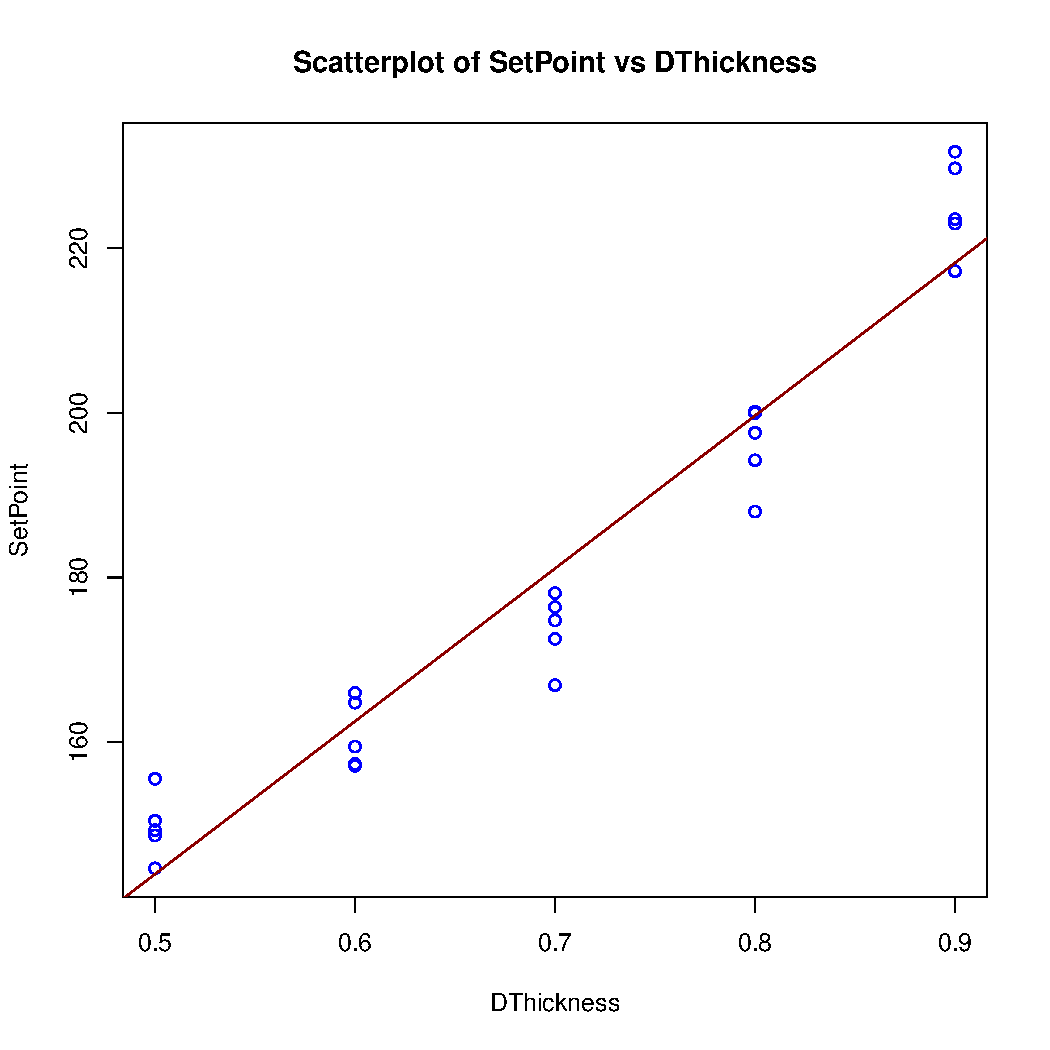
\includegraphics[width=7.5cm]{99_06_regrDThicknessSetPoint}
  \end{center}
\end{frame}

\begin{frame}[fragile]
  Regression analysis:\\
  \begin{small}
    \begin{verbatim}
Coefficients:
               Estimate Std. Error t value  p value    
(Intercept)      51.145      7.266   7.039 3.58e-07
DThickness      185.637     10.174  18.246 3.54e-15

Residual standard error: 7.194 on 23 degrees of freedom
Multiple R-squared: 0.9354,	Adjusted R-squared: 0.9326 
F-statistic: 332.9 on 1 and 23 DF,  p-value: 3.542e-15
    \end{verbatim}
  \end{small}
  Anderson-Darling test:\\
  \begin{small}
    \begin{verbatim}
A = 0.1865, p-value = 0.8949
    \end{verbatim}
  \end{small}
\end{frame}

\begin{frame}
  Regression line with confidence and prediction intervals at 95\% level:\\  
  \vspace{.3cm}
  \begin{center}
    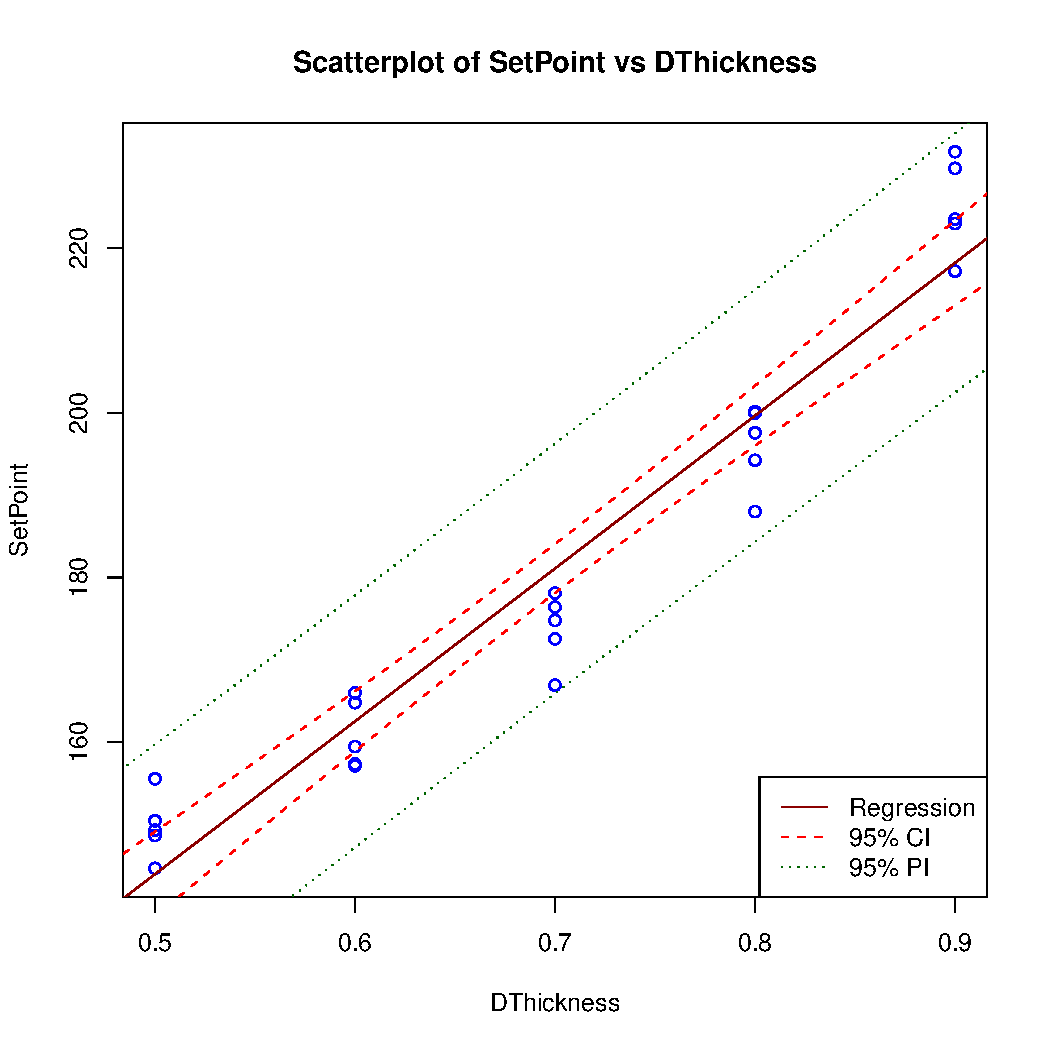
\includegraphics[width=6.5cm]{99_06_regrIntDThicknessSetPoint}
  \end{center}
\end{frame}

\begin{frame}
  Graphical check of the regression model:\\
  \vspace{.1cm}
  \begin{center}
    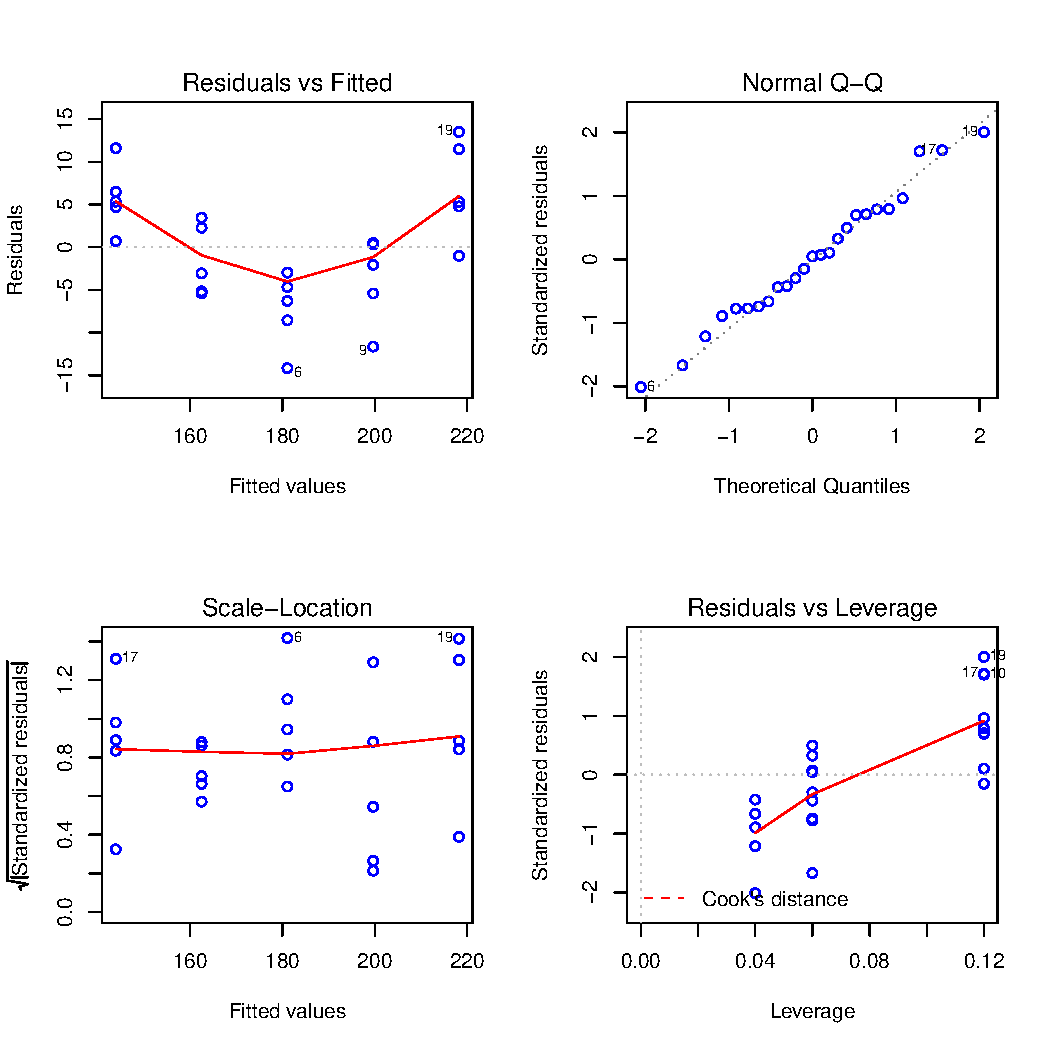
\includegraphics[width=7.5cm]{99_06_residDThicknessSetPoint}
    \end{center}
\end{frame}

\begin{frame}
  \begin{small}
    \begin{itemize}
      \item The relation that ``links'' the thickness of diaphragm with the pressure for which the switch trigs seems well described by a simple linear regression,  at least in the considered interval.
      \item The estimated formula is the follows: $ SetPoint = 51.145 + 185.637 \cdot DThickness $.
      \item The p-value for the significativity of the coefficient of \textit{DThickness} is extremely low. This fact confirms the  ``non random'' existing relation between the two variables.
      \item $ R^2 $ value is 0.9354. This fact confirms that the model explains well the observed data.
      \item The p-value of the estimate of the intercept is very low. The intercept is significative.
      \item The graphic of the residual values in respect of the estimated values shows a curvilinear trend. This fact implies that the model could be improved, for example with a quadratic model.
    \end{itemize}
  \end{small}
\end{frame}

\begin{frame}
  Scatterplot of the relation with polynomial regression curve:\\
  \vspace{.3cm}
  \begin{center}
    \includegraphics[width=6.5cm]{99_06_regrPolDThicknessSetPoint}
  \end{center}
\end{frame}

\begin{frame}[fragile]
  Polynomial regression analysis:\\
  \begin{small}
    \begin{verbatim}
Coefficients:
              Estimate Std. Error t value  p value
(Intercept)     202.47      26.24   7.717 1.07e-07
DThickness     -265.10      77.19  -3.434  0.00237
DThickness^2    321.96      54.94   5.860 6.76e-06

Residual standard error: 4.597 on 22 degrees of freedom
Multiple R-squared: 0.9748,	Adjusted R-squared: 0.9725 
F-statistic: 424.9 on 2 and 22 DF,  p-value: < 2.2e-16 
    \end{verbatim}
  \end{small}
  Anderson-Darling test:\\
  \begin{small}
    \begin{verbatim}
A = 0.4204, p-value = 0.3005
    \end{verbatim}
  \end{small}
\end{frame}

\begin{frame}
  Polynomial regression curve with a confidence and prediction interval at 95\% level:\\
  \vspace{.3cm}
  \begin{center}
    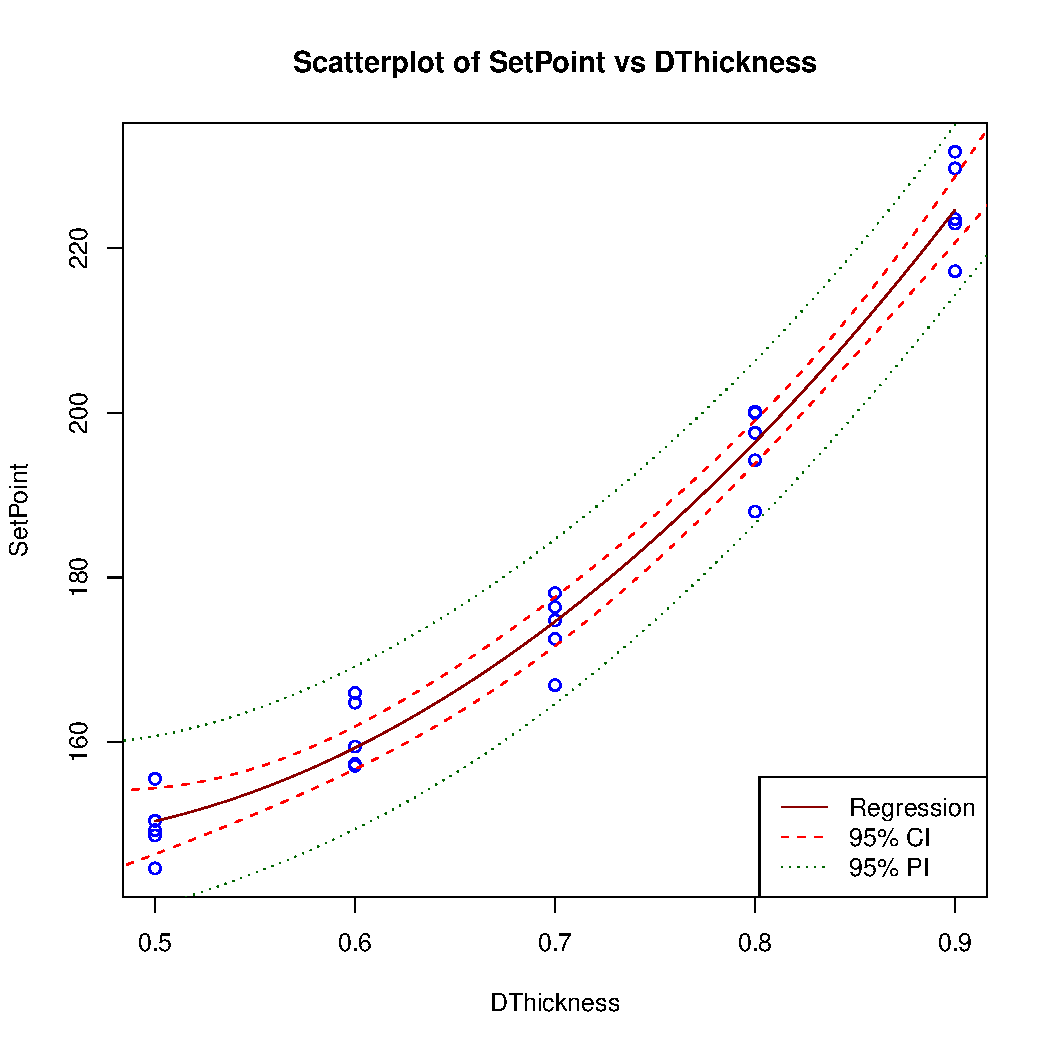
\includegraphics[width=6.5cm]{99_06_regrPolIntDThicknessSetPoint}
  \end{center}
\end{frame}

\begin{frame}
  \begin{small}
    \begin{itemize}
      \item The p-value of the quadratic term is significant, so the quadratic term explains a great quantity of variation in the response in respect of that explained by the linear model.
      \item The estimated formula is the follows: $ SetPoint = 202.47 - 265.10 \cdot DThickness + 321.96 \cdot DThickness^2 $.
      \item $ R^2 $ value is 0.9748, This value is certainly better than the same value of the simple linear model. 
      \item $ R^2 $ can never decrease. It will be always higher with the addiction of  predictors, even if the predictors addicted don't improve the model. 
      \item The value of the adjusted  $ R^2 $ allows one to compare models with different number of parameters.
      \item The value of the adjusted  $ R^2 $ of the polynomial model (0.9725) is greater than the same value of the simple linear model (0.9326).
    \end{itemize}
  \end{small}
\end{frame}

\begin{frame}
  Graphical check of the polynomial regression model:\\
  \vspace{.1cm}
  \begin{center}
    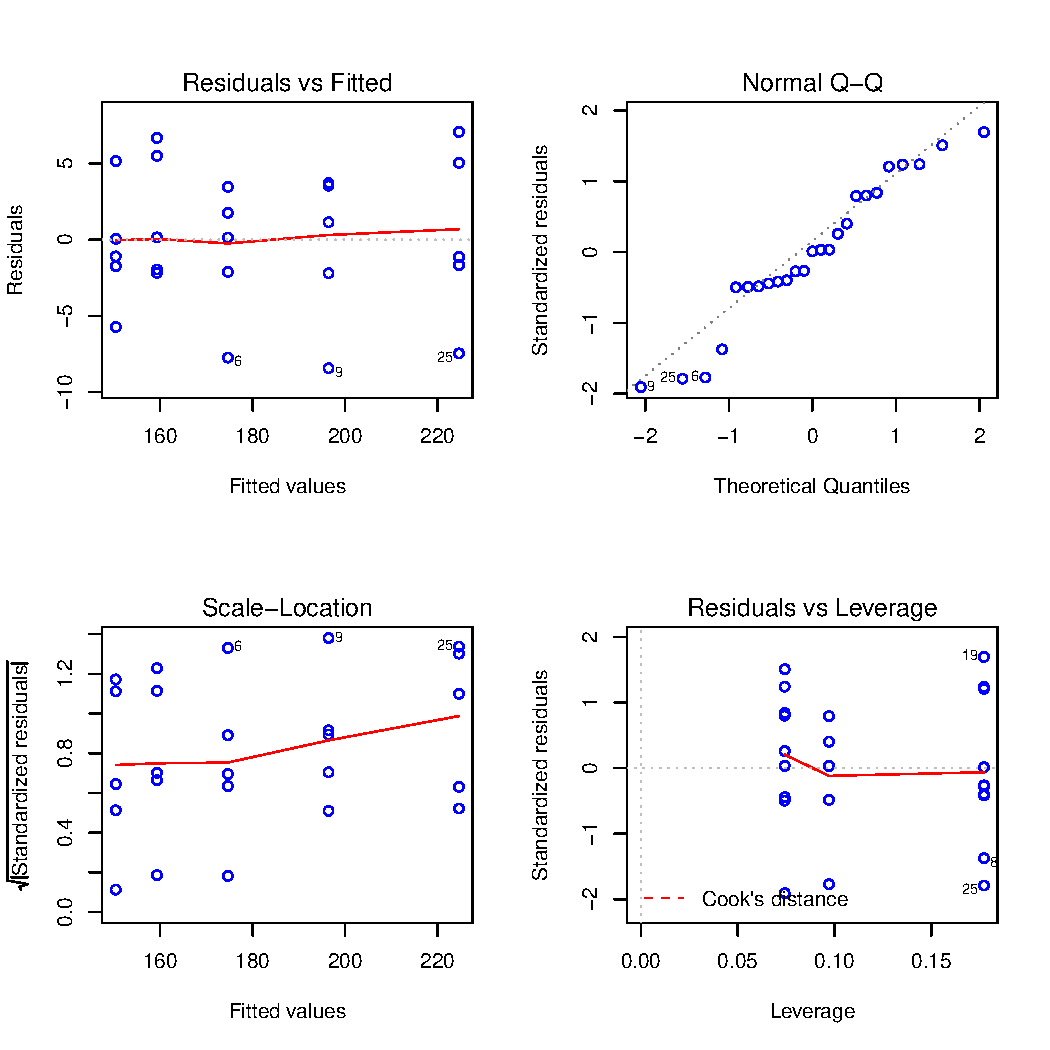
\includegraphics[width=7.5cm]{99_06_residPolDThicknessSetPoint}
    \end{center}
\end{frame}

\begin{frame}
  \vspace{0.75cm}
  \begin{itemize}
    \item The graphic of the estimated values vs residuals doesn't show any systematic trend of the residuals and the variance seems to be the same for each estimated value.
    \vspace{0.5cm}
    \item The residuals are quite well aligned on the line representing the quantile of the normal distribution: It is reasonable to assume that they are then normally distributed.
  \end{itemize}
\end{frame}

\begin{frame}
  \begin{floatingfigure}[l]{7cm}
    \vspace{-1cm}
    \centering
    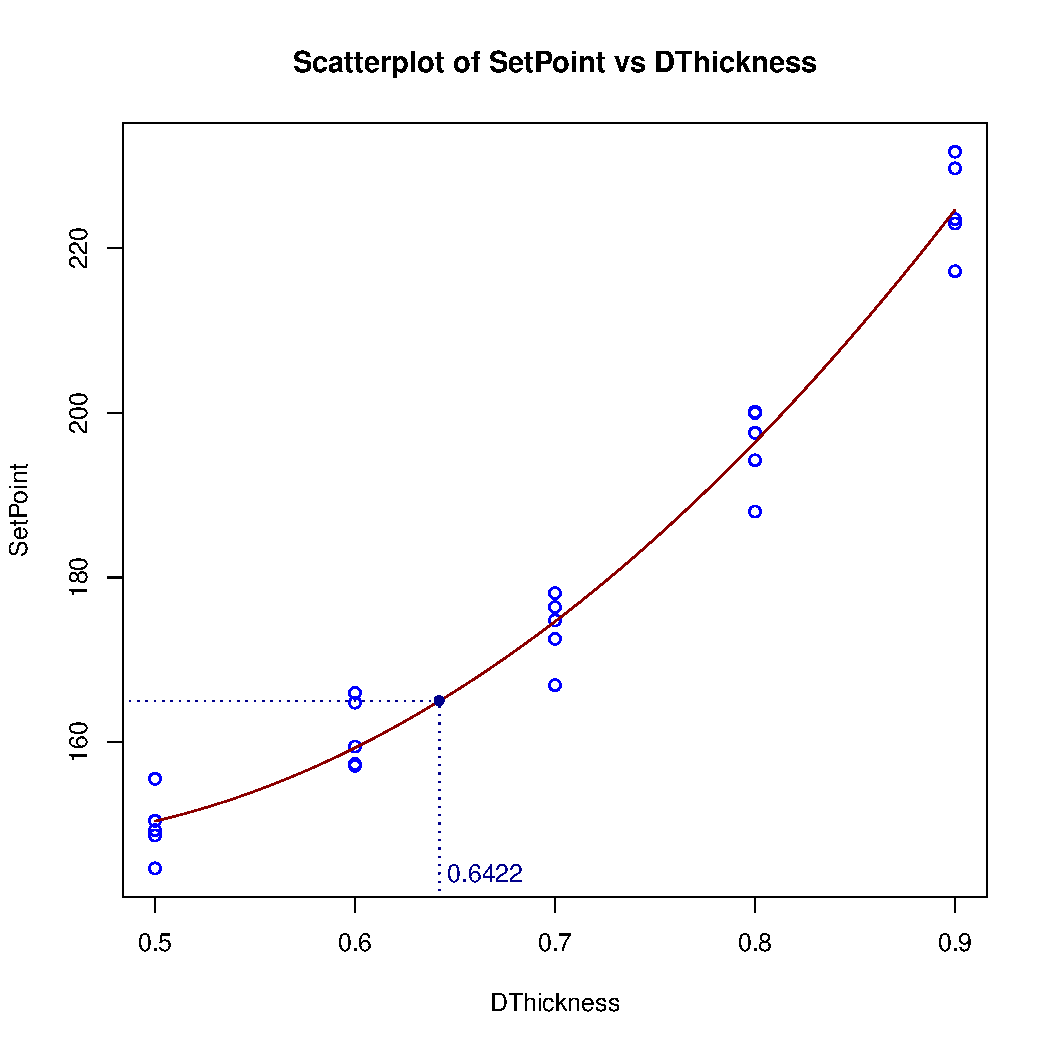
\includegraphics[width=7.5cm]{99_06_regrPol165DThicknessSetPoint}\\
  \end{floatingfigure}
  \begin{footnotesize}
    \vspace{1cm}
    Using the quadratic regression model, the best choice for the thickness of diaphragm is approximately 0.64 mm. This result is obtained replacing 165 for \textit{SetPoint} (y) in the regression model and solving the thickness (\textit{DThickness} (x) using a quadratic equation.
  \end{footnotesize}
\end{frame}

\livelloB{Antierosion screens}

\begin{frame}
  \begin{description}
    \item[Data: ]erosion.txt \\ 
    \item[Description: ]
      \begin{footnotesize}
        \begin{itemize}
	  \item \textit{Hardness}: indicates the hardness of the turbine;
          \item \textit{Abrasion}: indicates the abrasion.
        \end{itemize}
      \end{footnotesize}
    \item[Aims: ]
      \begin{footnotesize}
        A builder of turbines wants to know how an antierosion screen is able to resist the abrasive action during use. The direct measurement of abrasion is difficult, expensive and destructive. However, the builder hopes to produce an abrasion resistance using the hardness of the steel. The loss due to abrasion and the hardness were measured on 24 antierosion screens, chosen randomly.   
        \begin{itemize}
          \item[-] Let us graphically represent the relation between the variables.
          \item[-] Let us compute a simple linear regression between the variables.
          \item[-] Let us try to introduce the terms of second and third degree in the model.
        \end{itemize}
      \end{footnotesize}
  \end{description}
\end{frame}

\begin{frame}
  Scatterplot:\\
  \vspace{.3cm}
  \begin{center}
    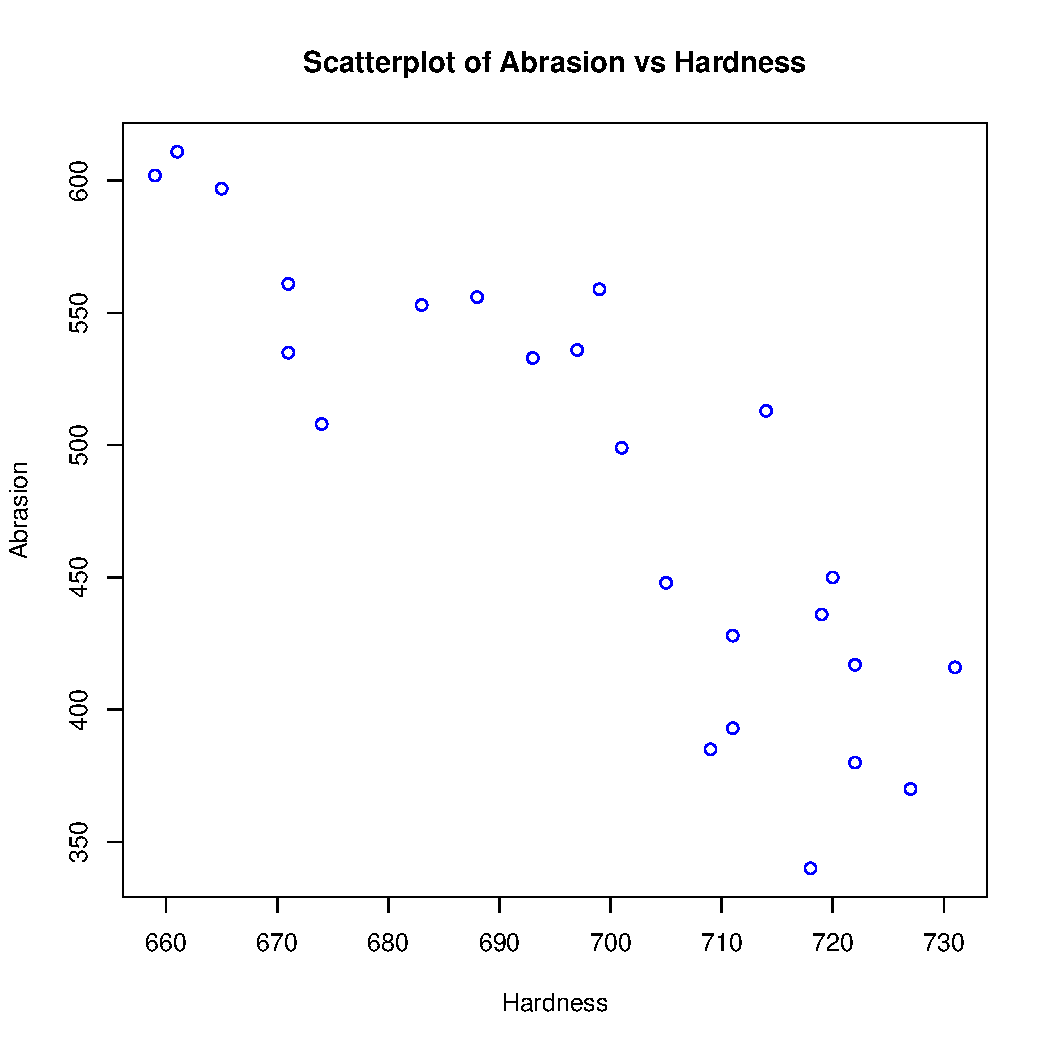
\includegraphics[width=7.5cm]{99_06_scattHardnessAbrasion}
  \end{center}
\end{frame}

\begin{frame}
  Regression line:\\
  \vspace{.3cm}
  \begin{center}
    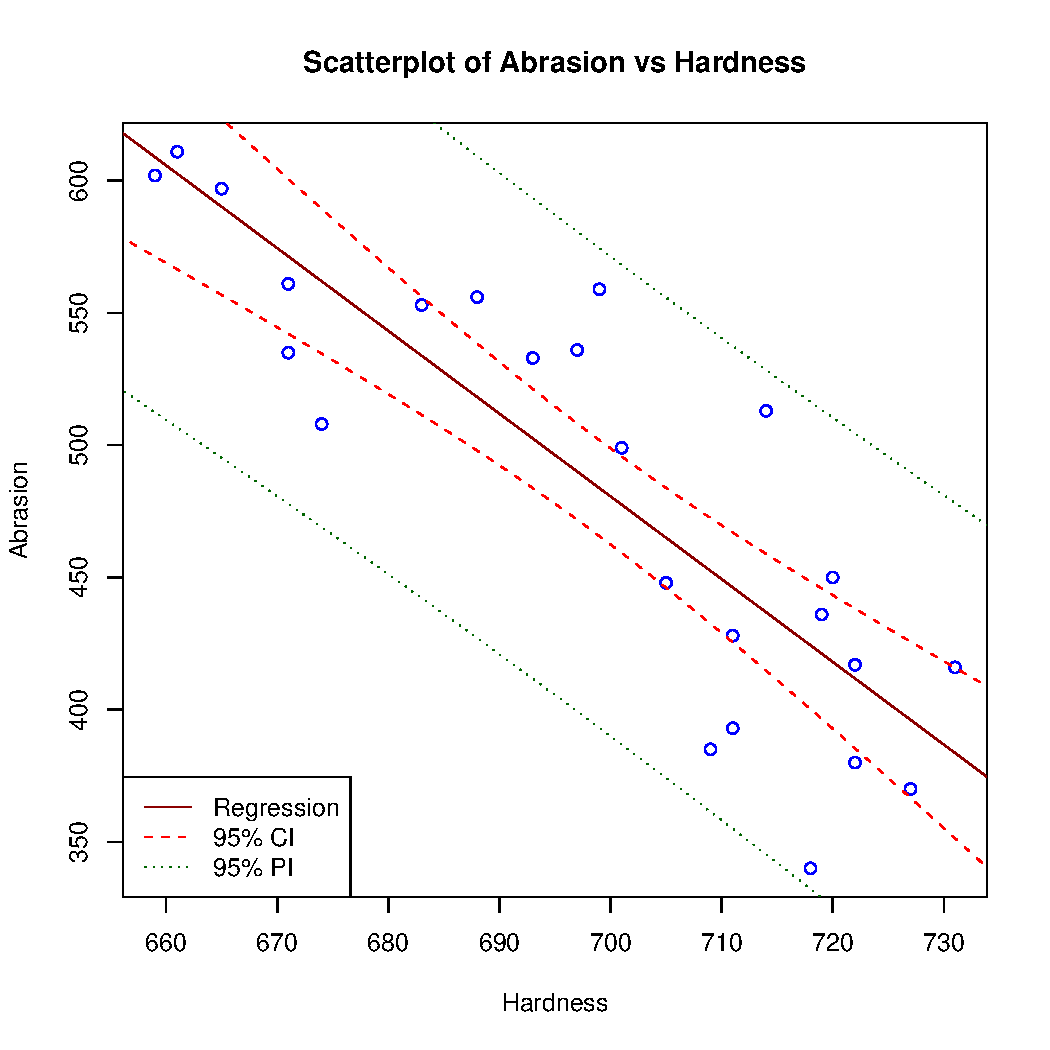
\includegraphics[width=7.5cm]{99_06_regrIntHardnessAbrasion}
  \end{center}
\end{frame}

\begin{frame}[fragile]
  Regression analysis:\\
  \begin{small}
    \begin{verbatim}
Coefficients:
             Estimate Std. Error t value  p value   
(Intercept) 2671.0980   279.0055   9.574 2.65e-09
x             -3.1292     0.3991  -7.841 8.22e-08

Residual standard error: 42.85 on 22 degrees of freedom
Multiple R-squared: 0.7365,	Adjusted R-squared: 0.7245 
F-statistic: 61.49 on 1 and 22 DF,  p-value: 8.22e-08 
    \end{verbatim}
  \end{small}
  Anderson-Darling test:\\
  \begin{small}
    \begin{verbatim}
A = 0.1559, p-value = 0.9471
    \end{verbatim}
  \end{small}
\end{frame}

\begin{frame}
  Graphical check of the model:\\
  \vspace{.3cm}
  \begin{center}
    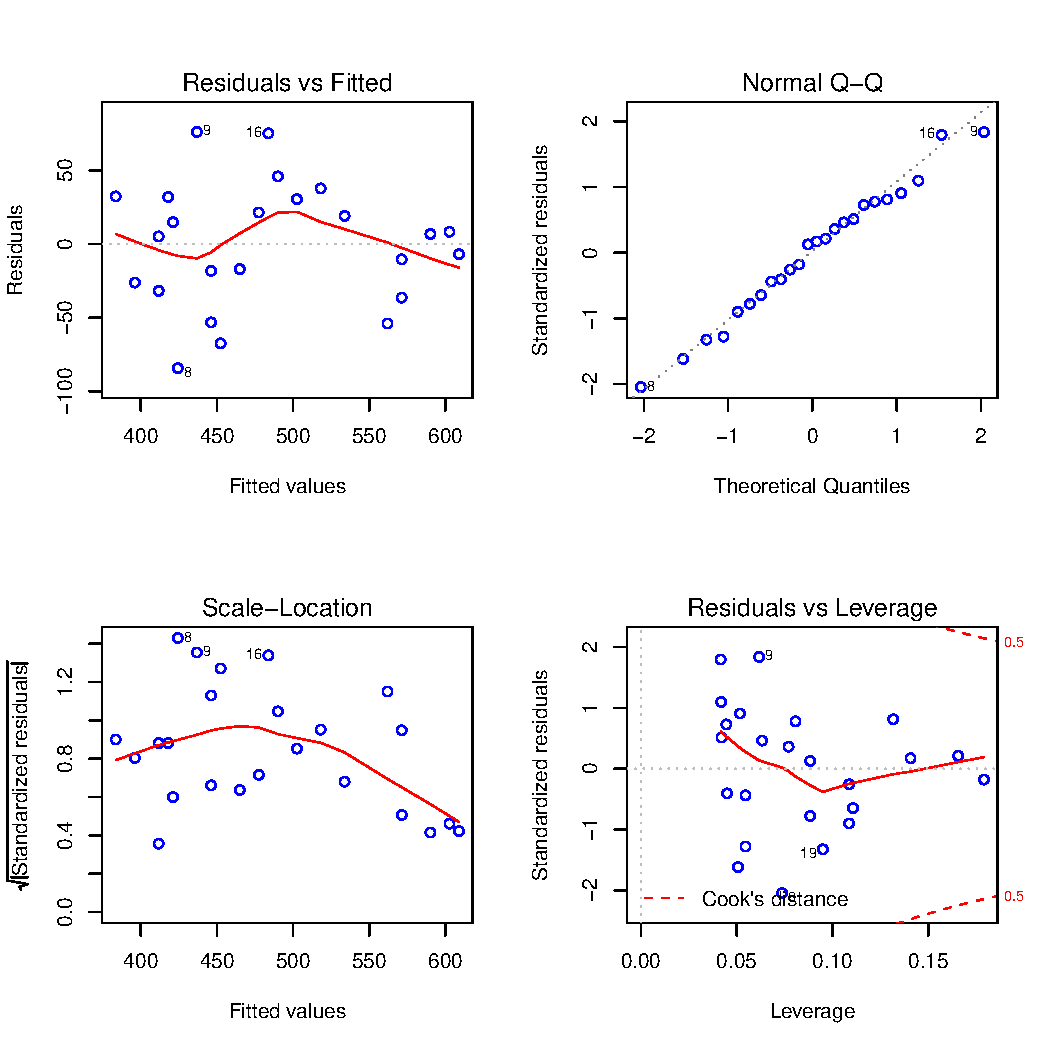
\includegraphics[width=7.5cm]{99_06_residHardnessAbrasion}
  \end{center}
\end{frame}

\begin{frame}
  Quadratic regression curve:\\
  \vspace{.3cm}
  \begin{center}
    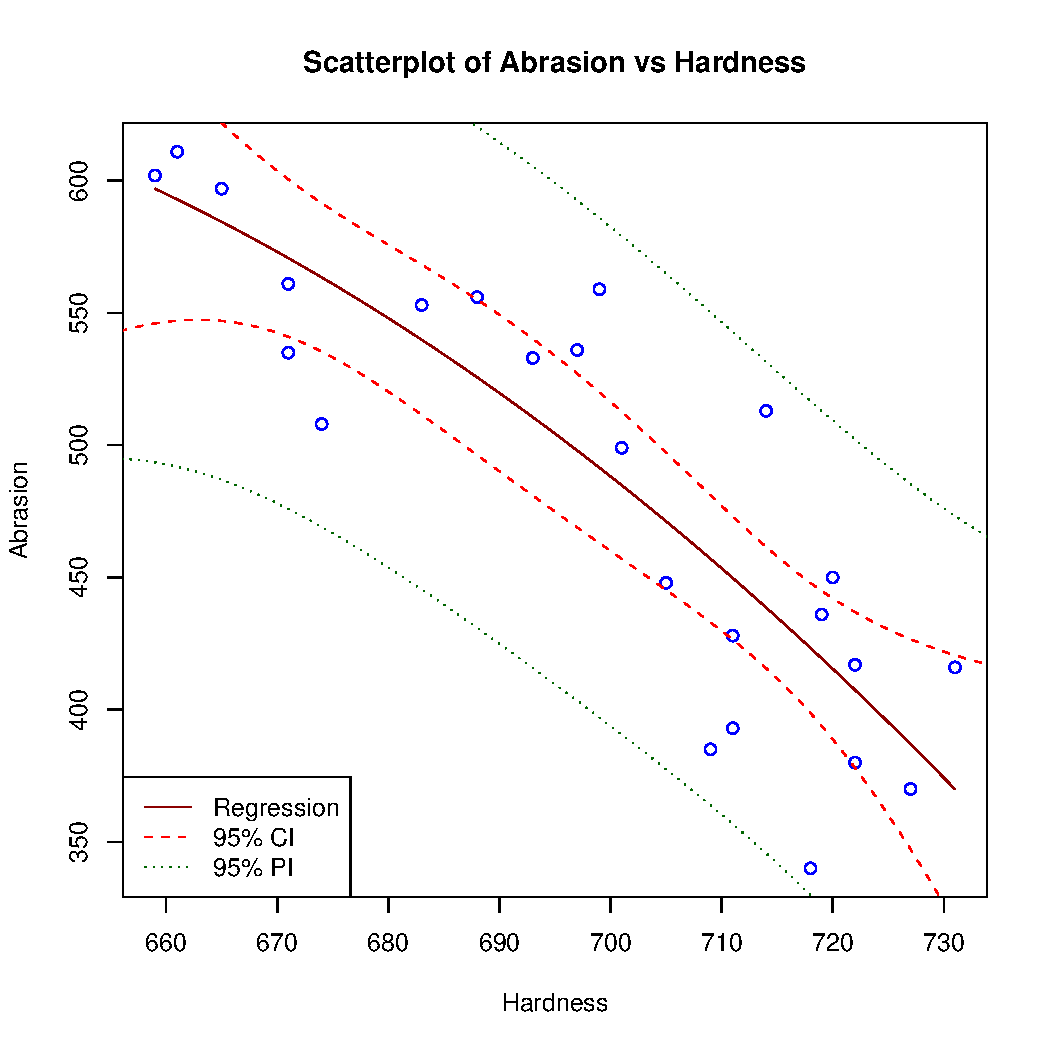
\includegraphics[width=7.5cm]{99_06_regrQuadIntHardnessAbrasion}
  \end{center}
\end{frame}

\begin{frame}[fragile]
  Regression analysis:\\
  \begin{small}
    \begin{verbatim}
Coefficients:
              Estimate Std. Error t value  p value
(Intercept) -5.095e+03  1.055e+04  -0.483    0.634
x            1.927e+01  3.041e+01   0.634    0.533
x^2         -1.613e-02  2.190e-02  -0.737    0.470

Residual standard error: 43.3 on 21 degrees of freedom
Multiple R-squared: 0.7431,	Adjusted R-squared: 0.7187 
F-statistic: 30.37 on 2 and 21 DF,  p-value: 6.342e-07 
    \end{verbatim}
  \end{small}
  Anderson-Darling test:\\
  \begin{small}
    \begin{verbatim}
A = 0.2841, p-value = 0.6
    \end{verbatim}
  \end{small}
\end{frame}

\begin{frame}
  Graphical check of the model:\\
  \vspace{.3cm}
  \begin{center}
    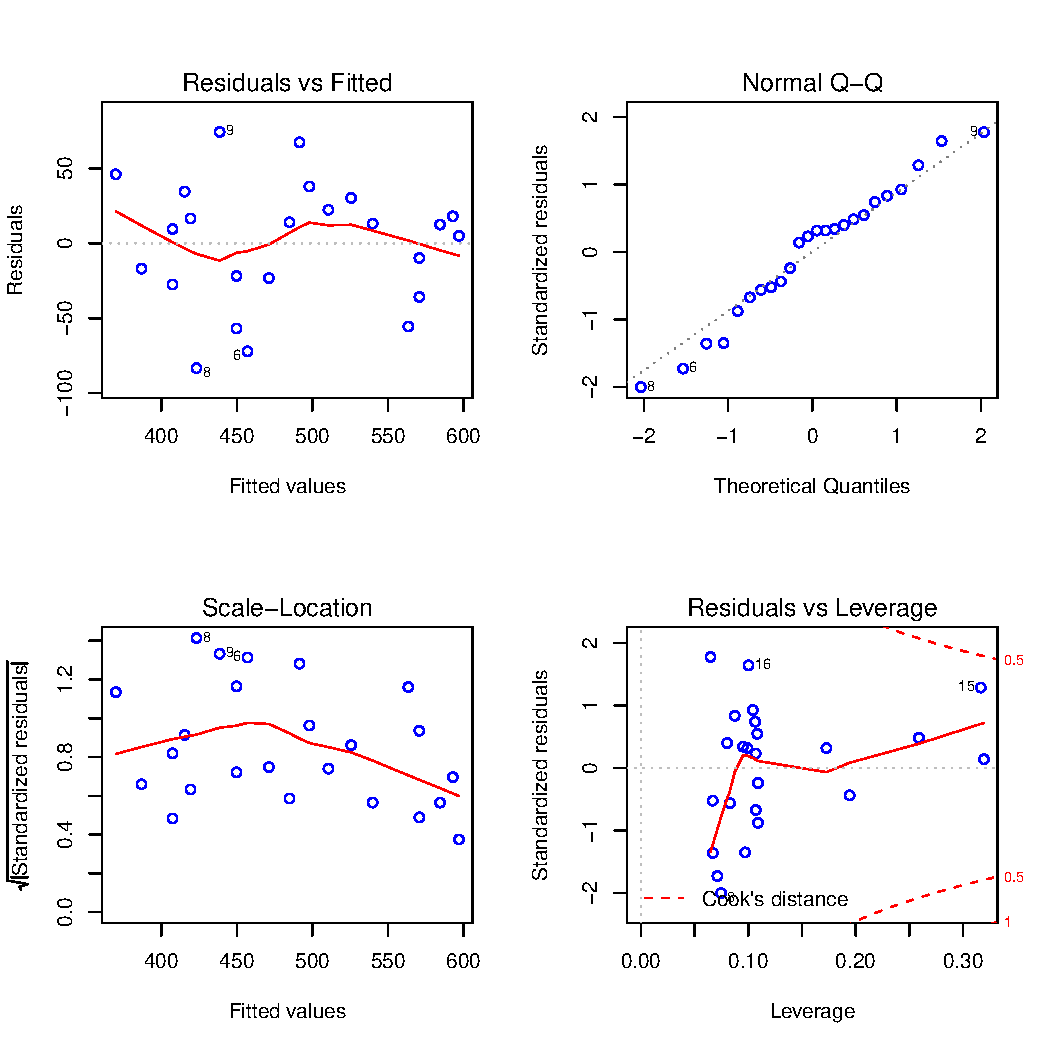
\includegraphics[width=7.5cm]{99_06_residQuadHardnessAbrasion}
  \end{center}
\end{frame}

\begin{frame}
  Cubic regression curve:\\
  \vspace{.3cm}
  \begin{center}
    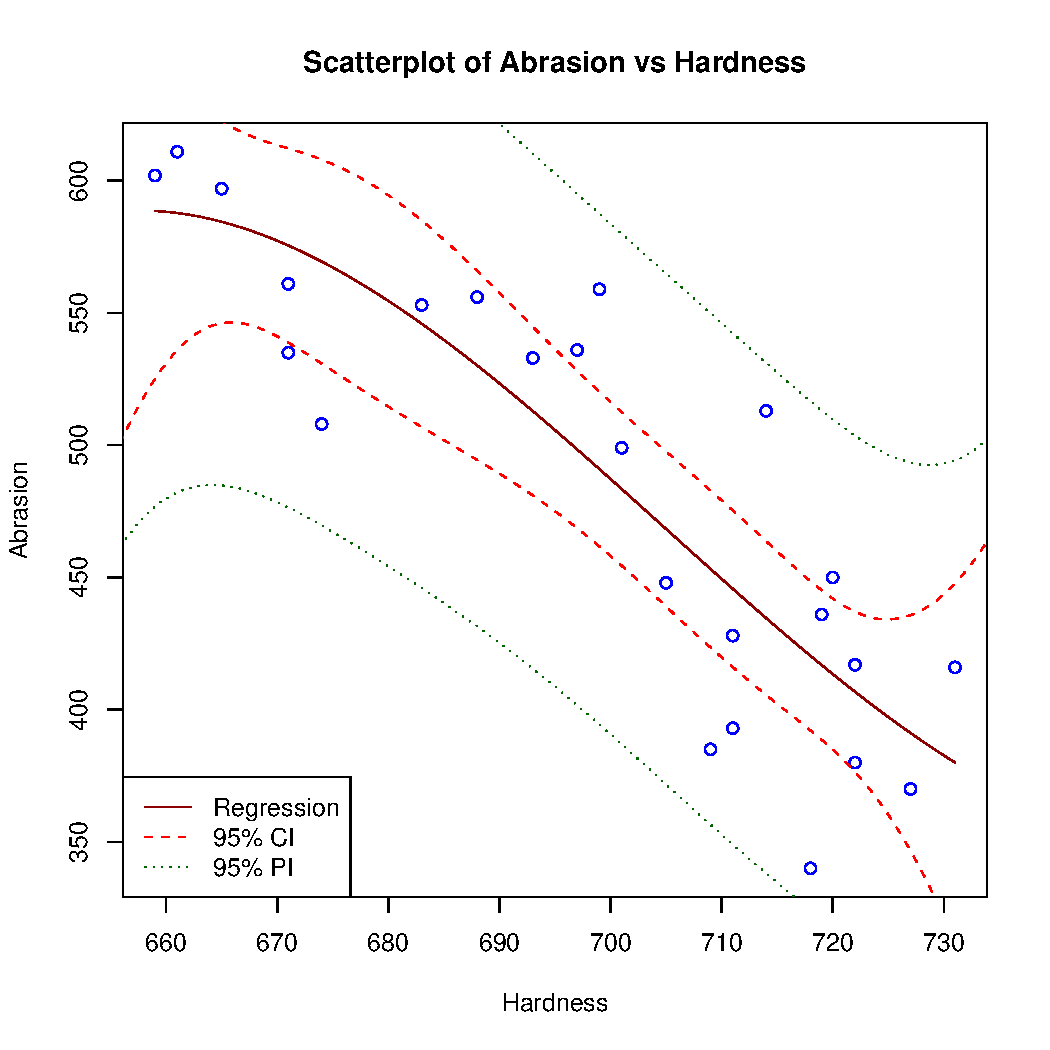
\includegraphics[width=7.5cm]{99_06_regrCubIntHardnessAbrasion}
  \end{center}
\end{frame}

\begin{frame}[fragile]
  Regression analysis:\\
  \begin{small}
    \begin{verbatim}
Coefficients:
              Estimate Std. Error t value  p value
(Intercept) -1.955e+05  3.938e+05  -0.496    0.625
x            8.416e+02  1.701e+03   0.495    0.626
x^2         -1.200e+00  2.448e+00  -0.490    0.629
x^3          5.675e-04  1.174e-03   0.484    0.634

Residual standard error: 44.12 on 20 degrees of freedom
Multiple R-squared: 0.7461,	Adjusted R-squared: 0.708 
F-statistic: 19.59 on 3 and 20 DF,  p-value: 3.615e-06 
    \end{verbatim}
  \end{small}
  Anderson-Darling test:\\
  \begin{small}
    \begin{verbatim}
A = 0.3706, p-value = 0.3958
    \end{verbatim}
  \end{small}
\end{frame}

\begin{frame}
  Graphical check of the model:\\
  \vspace{.3cm}
  \begin{center}
    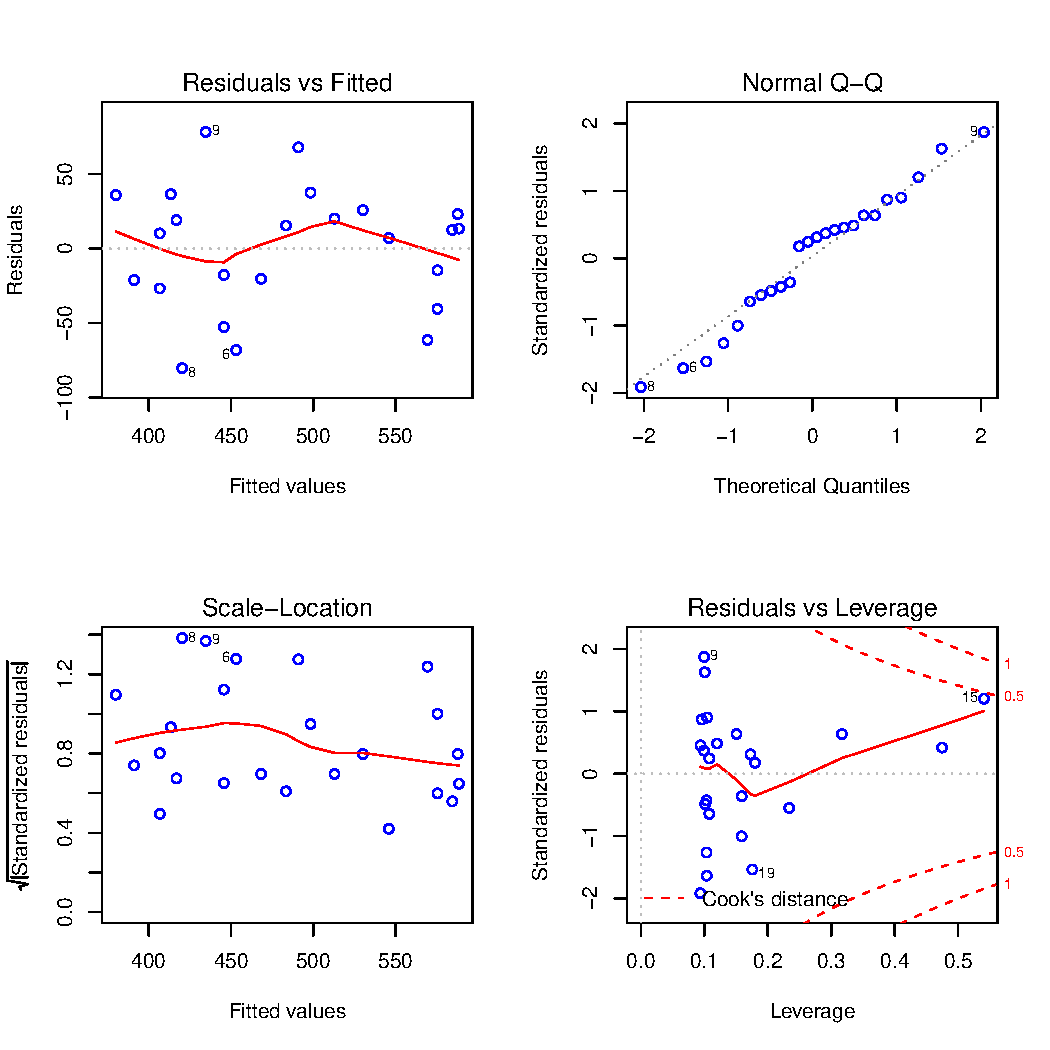
\includegraphics[width=7.5cm]{99_06_residCubHardnessAbrasion}
  \end{center}
\end{frame}

\livelloB{Emissions from diesel trucks}

\begin{frame}
  \begin{description}
    \item[Data: ]diesel.txt \\ 
    \item[Description: ]
      \begin{footnotesize}
        \begin{itemize}
          \item \textit{NOx}: indicates the emissions of nitrogen oxide;
          \item \textit{Humidity}: indicates the percentage of humidity.
        \end{itemize}
      \end{footnotesize}
      \begin{tiny}
       The data derive from a study on the influence of weather conditions on pollutant emissions.	
      \end{tiny}
    \item[Aims: ]
      \begin{footnotesize}
        Let us analyse the effects of humidity on the emissions of the diesel trucks.
        \begin{itemize}
          \item[-] Let us graphically represent the relation between the variables.
          \item[-] Let us compute a simple linear regression between variables.
          \item[-] Let us try to introduce the terms of second and third degree in the model.
        \end{itemize}
      \end{footnotesize}
  \end{description}
\end{frame}

\begin{frame}
  Scatterplot:\\
  \vspace{.3cm}
  \begin{center}
    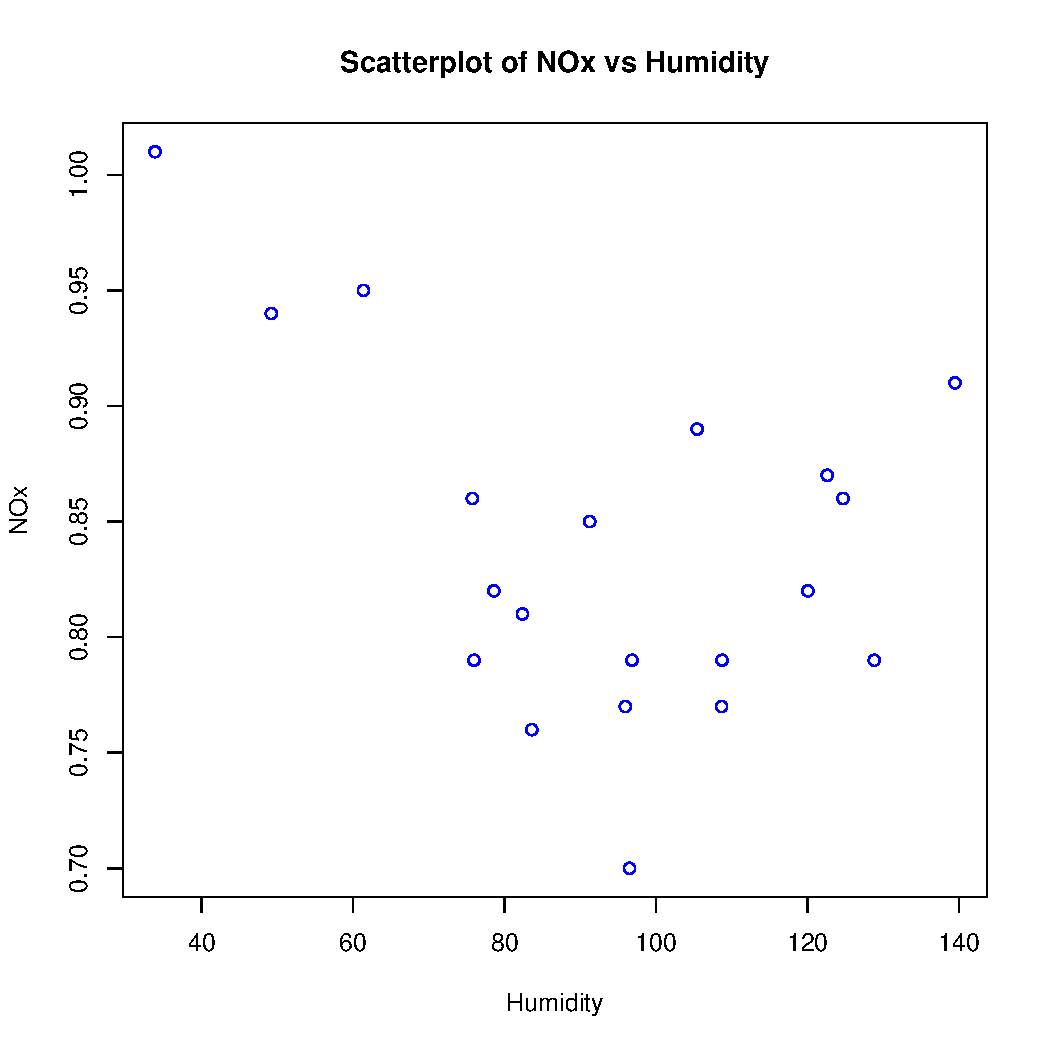
\includegraphics[width=7.5cm]{99_06_scattHumidityNOx}
  \end{center}
\end{frame}

\begin{frame}
  Regression line:\\
  \vspace{.3cm}
  \begin{center}
    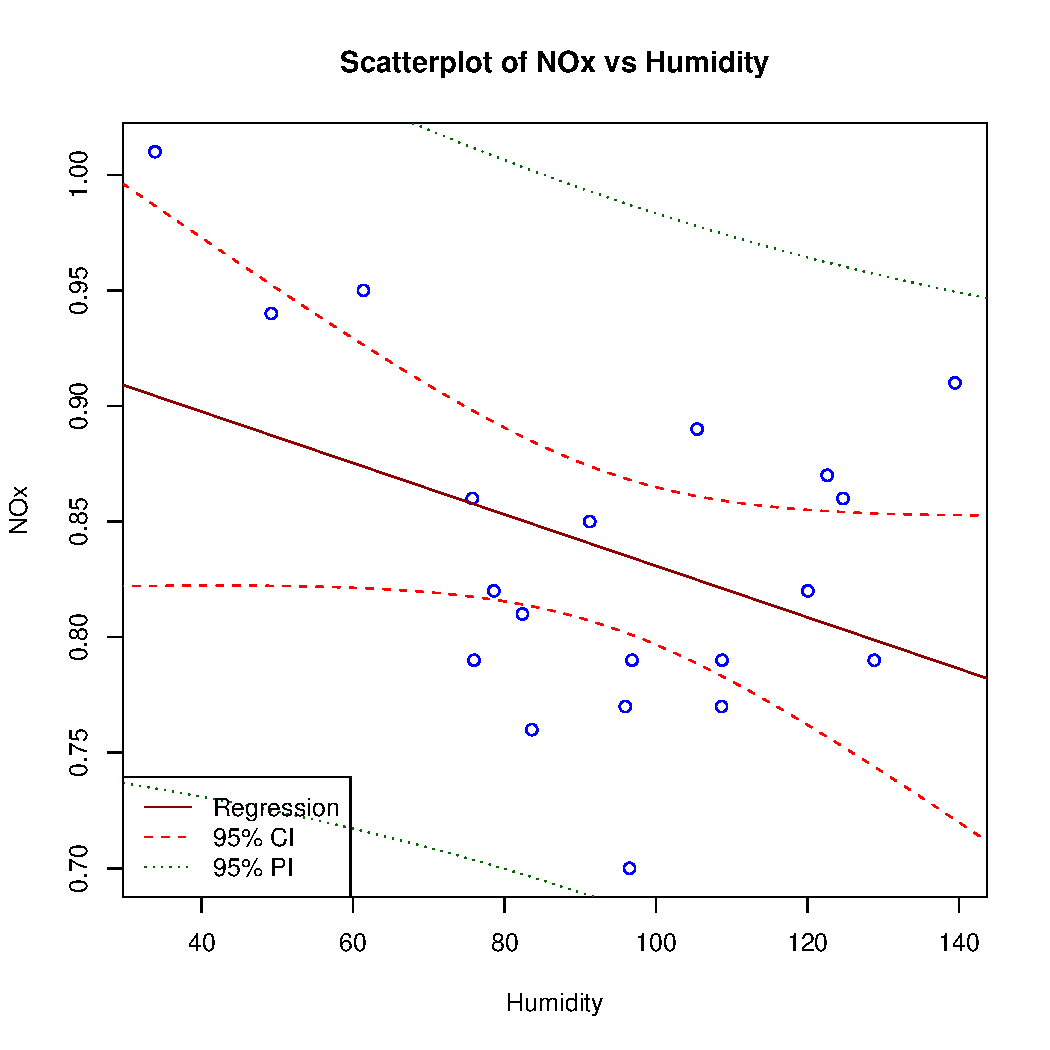
\includegraphics[width=7.5cm]{99_06_regrIntHumidityNOx}
  \end{center}
\end{frame}

\begin{frame}[fragile]
  Regression analysis:\\
  \begin{small}
    \begin{verbatim}
Coefficients:
              Estimate Std. Error t value  p value   
(Intercept)  0.9420426  0.0581198  16.209  3.5e-12
x           -0.0011124  0.0005951  -1.869    0.078

Residual standard error: 0.07074 on 18 degrees of freedom
Multiple R-squared: 0.1626,	Adjusted R-squared: 0.116 
F-statistic: 3.494 on 1 and 18 DF,  p-value: 0.07794 
    \end{verbatim}
  \end{small}
  Anderson-Darling test:\\
  \begin{small}
    \begin{verbatim}
A = 0.264, p-value = 0.6596
    \end{verbatim}
  \end{small}
\end{frame}

\begin{frame}
  Graphical check of the model:\\
  \vspace{.3cm}
  \begin{center}
    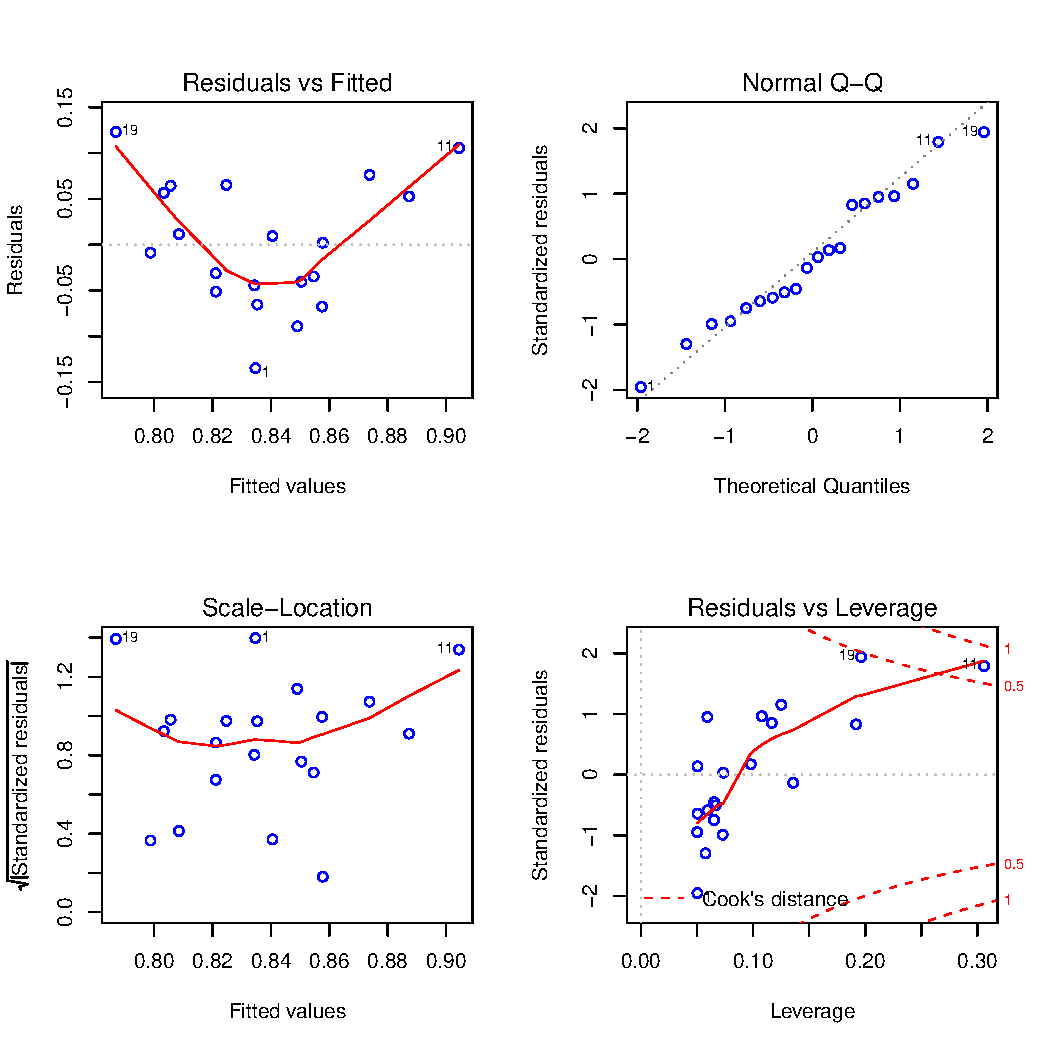
\includegraphics[width=7.5cm]{99_06_residHumidityNOx}
  \end{center}
\end{frame}

\begin{frame}
  Quadratic regression curve:\\
  \vspace{.3cm}
  \begin{center}
    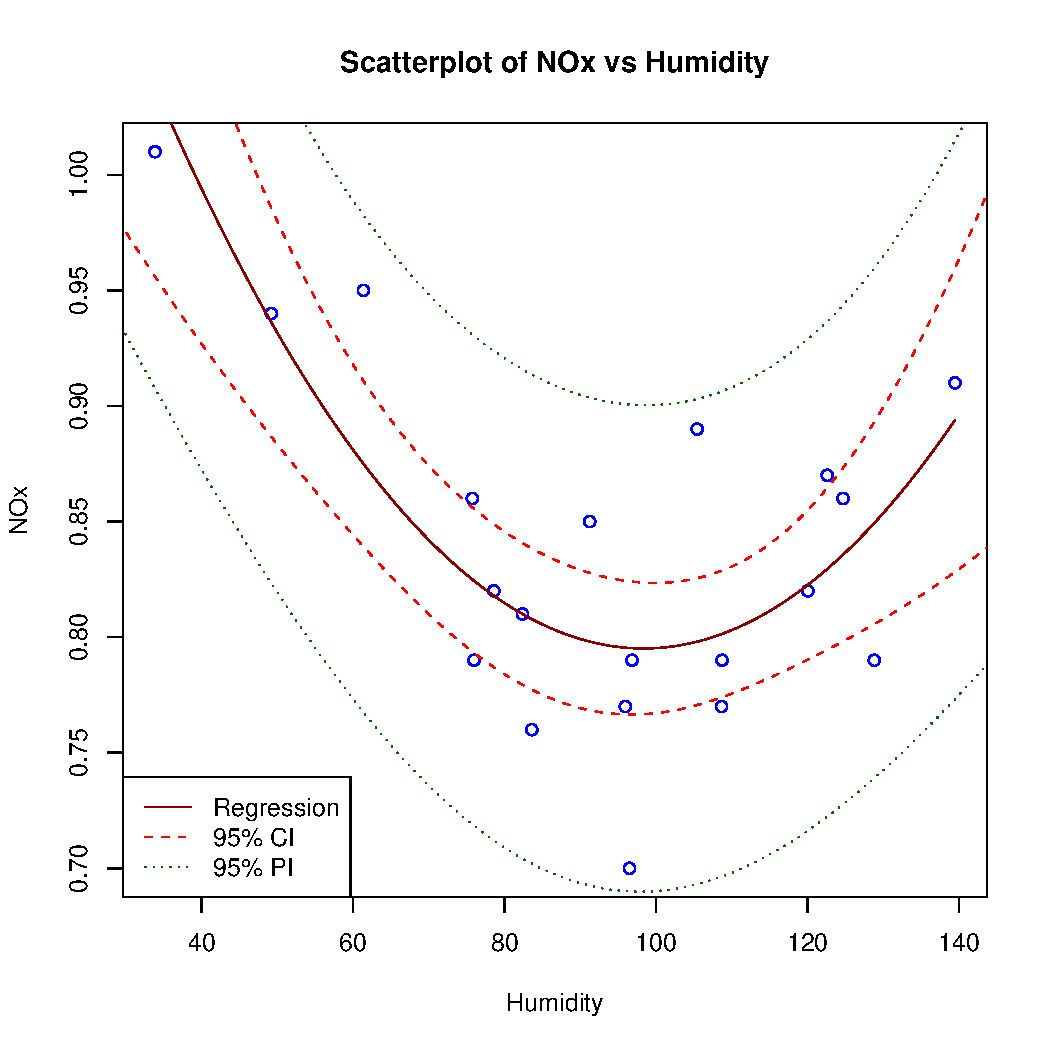
\includegraphics[width=7.5cm]{99_06_regrQuadIntHumidityNOx}
  \end{center}
\end{frame}

\begin{frame}[fragile]
  Regression analysis:\\
  \begin{small}
    \begin{verbatim}
Coefficients:
             Estimate Std. Error t value  p value   
(Intercept) 1.360e+00  9.729e-02  13.980 9.42e-11
x          -1.149e-02  2.244e-03  -5.119 8.55e-05
x^2         5.841e-05  1.243e-05   4.700 0.000206

Residual standard error: 0.048 on 17 degrees of freedom
Multiple R-squared: 0.6358,	Adjusted R-squared: 0.593 
F-statistic: 14.84 on 2 and 17 DF,  p-value: 0.0001867 
    \end{verbatim}
  \end{small}
  Anderson-Darling test:\\
  \begin{small}
    \begin{verbatim}
A = 0.1576, p-value = 0.9425
    \end{verbatim}
  \end{small}
\end{frame}

\begin{frame}
  Graphical check of the model:\\
  \vspace{.3cm}
  \begin{center}
    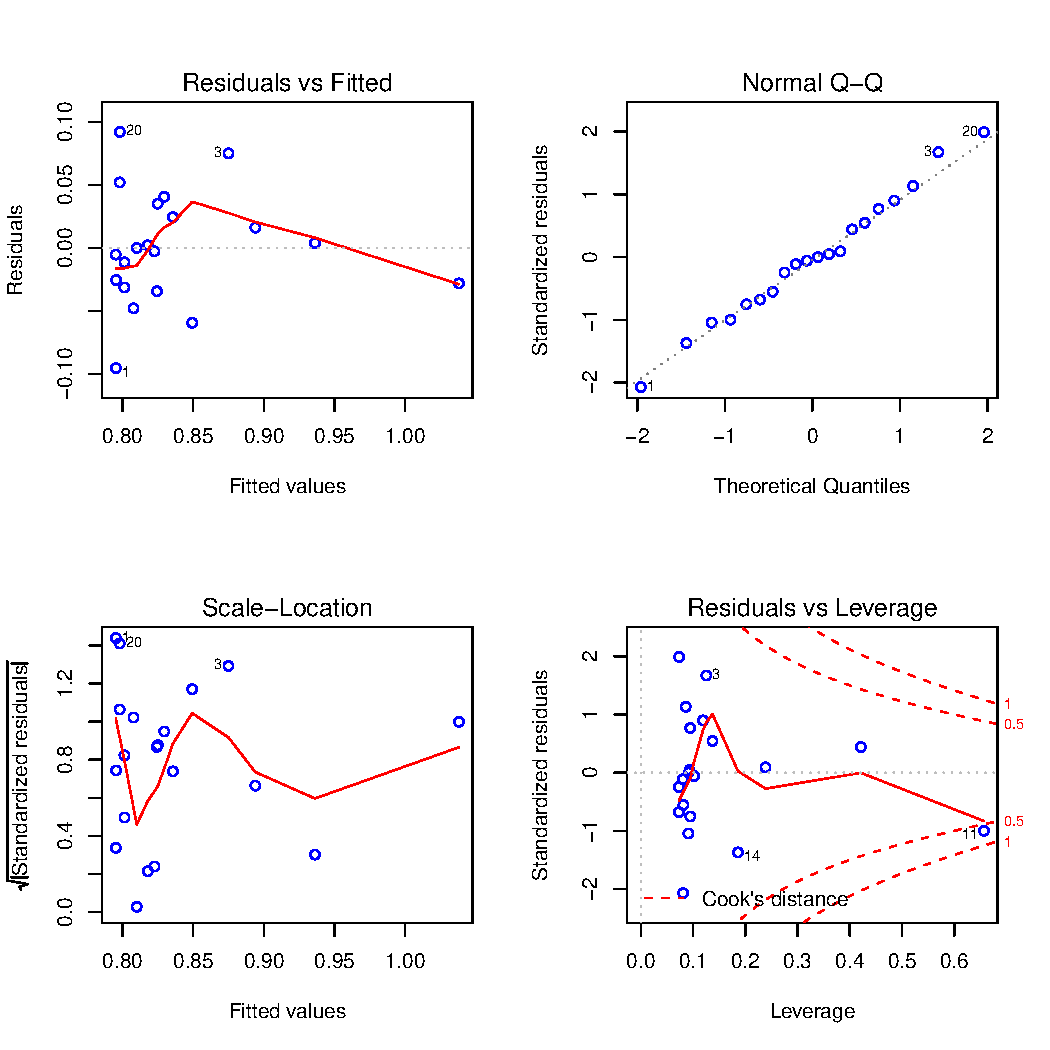
\includegraphics[width=7.5cm]{99_06_residQuadHumidityNOx}
  \end{center}
\end{frame}

\begin{frame}
  Cubic regression curve:\\
  \vspace{.3cm}
  \begin{center}
    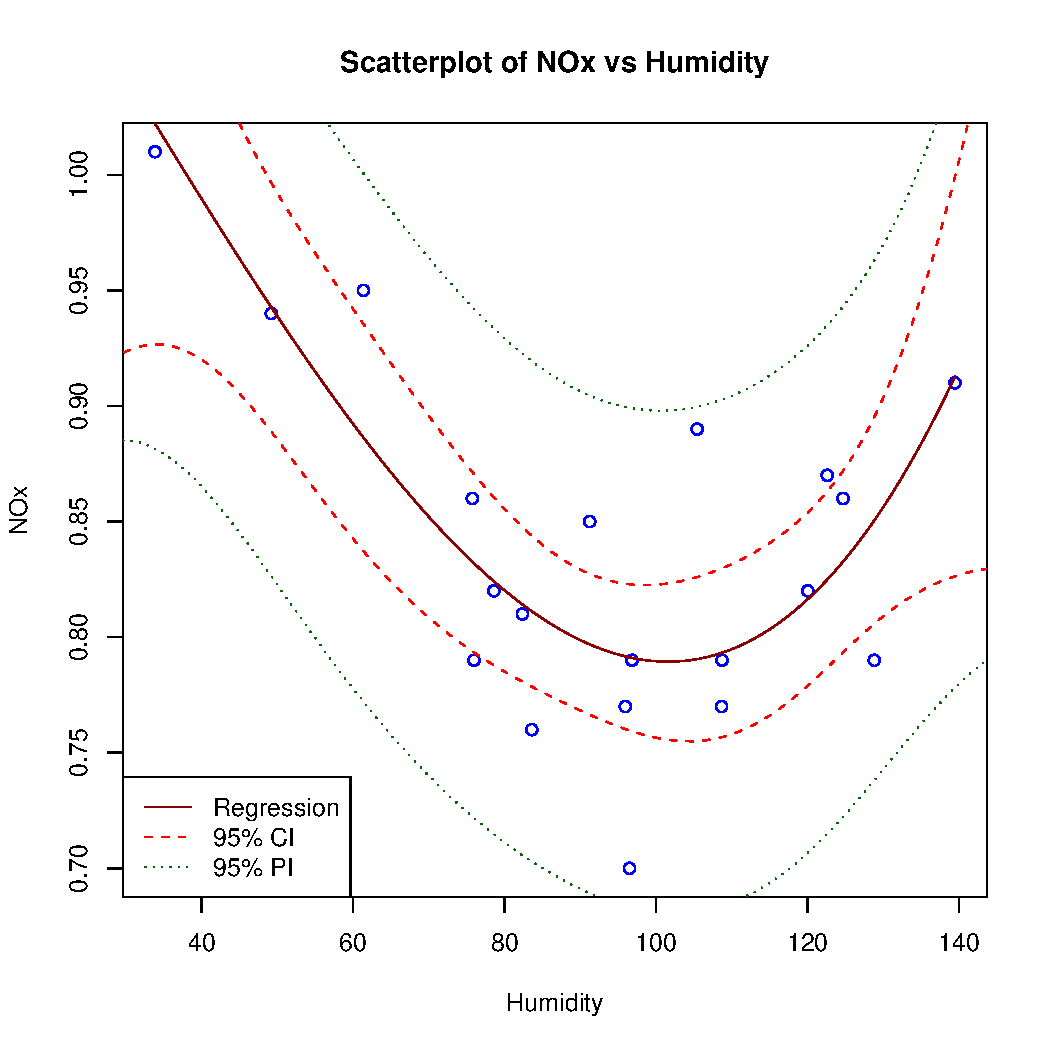
\includegraphics[width=7.5cm]{99_06_regrCubIntHumidityNOx}
  \end{center}
\end{frame}

\begin{frame}[fragile]
  Regression analysis:\\
  \begin{small}
    \begin{verbatim}
Coefficients:
             Estimate Std. Error t value  p value   
(Intercept) 1.196e+00  2.442e-01   4.899 0.000161
x          -4.565e-03  9.716e-03  -0.470 0.644807    
x^2        -2.841e-05  1.191e-04  -0.239 0.814492    
x^3         3.339e-07  4.554e-07   0.733 0.474107

Residual standard error: 0.04867 on 16 degrees of freedom
Multiple R-squared: 0.6477,	Adjusted R-squared: 0.5816 
F-statistic: 9.804 on 3 and 16 DF,  p-value: 0.000657
    \end{verbatim}
  \end{small}
  Anderson-Darling test:\\
  \begin{small}
    \begin{verbatim}
A = 0.3708, p-value = 0.3892
    \end{verbatim}
  \end{small}
\end{frame}

\begin{frame}
  Graphical check of the model:\\
  \vspace{.3cm}
  \begin{center}
    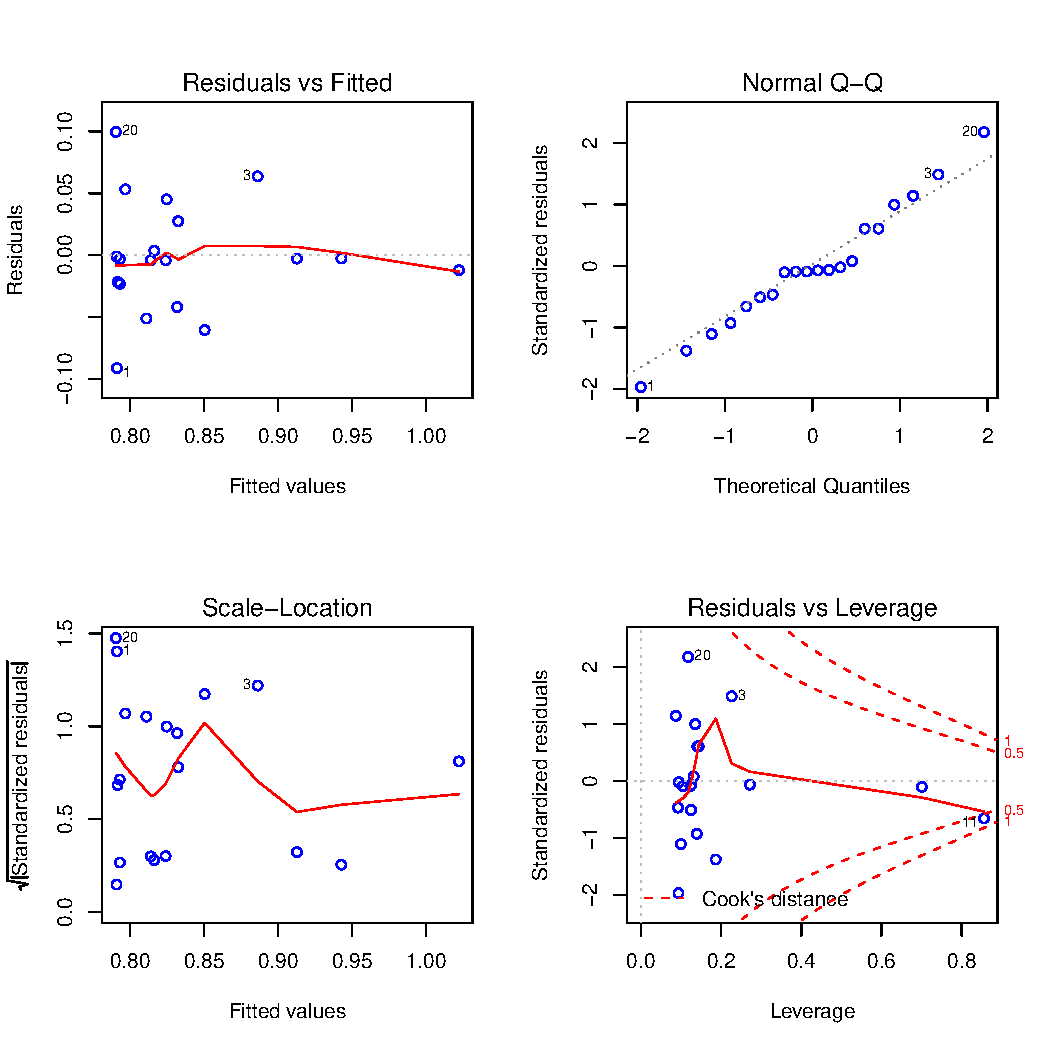
\includegraphics[width=7.5cm]{99_06_residCubHumidityNOx}
  \end{center}
\end{frame}



\livelloA{Multiple regression}

\livelloB{Knocking of the engine}

\begin{frame}
  \begin{description}
    \item[Data: ]knock.txt \\ 
    \item[Description: ]
      \begin{footnotesize}
        \begin{itemize}
          \item \textit{Spark}: indicates the time of advance of the spark plug ignition;
          \item \textit{AFR}: indicates the air fuel ratio (Air Fuel Ratio);
          \item \textit{Intake}: indicates the inlet temperature;
          \item \textit{Exhaust}: indicates the exhaust temperature;
          \item \textit{Knock}: indicates the knocking of the engine.
        \end{itemize}
      \end{footnotesize}
    \item[Aims: ]
      \begin{footnotesize}
        The engeneers want to reduce the knocking of the engines. Before doing this, they have to identify which variables influence this phenomenon. Data are randomly collected from 13 engines.
        \begin{itemize}
          \item[-] Let us graphically represent the relations between \textit{Knock} and the predictors and let us compute the correlation.
          \item[-] Let us compute a multiple linear regression between \textit{Knock} and the predictors.
          \item[-] Is It possible to improve the resulting model? How?
        \end{itemize}
      \end{footnotesize}
  \end{description}
\end{frame}

\begin{frame}
  Scatterplot matrix of the relations between measures with correlations and significativity: \\
  \vspace{-0.3cm}
  \begin{center}
    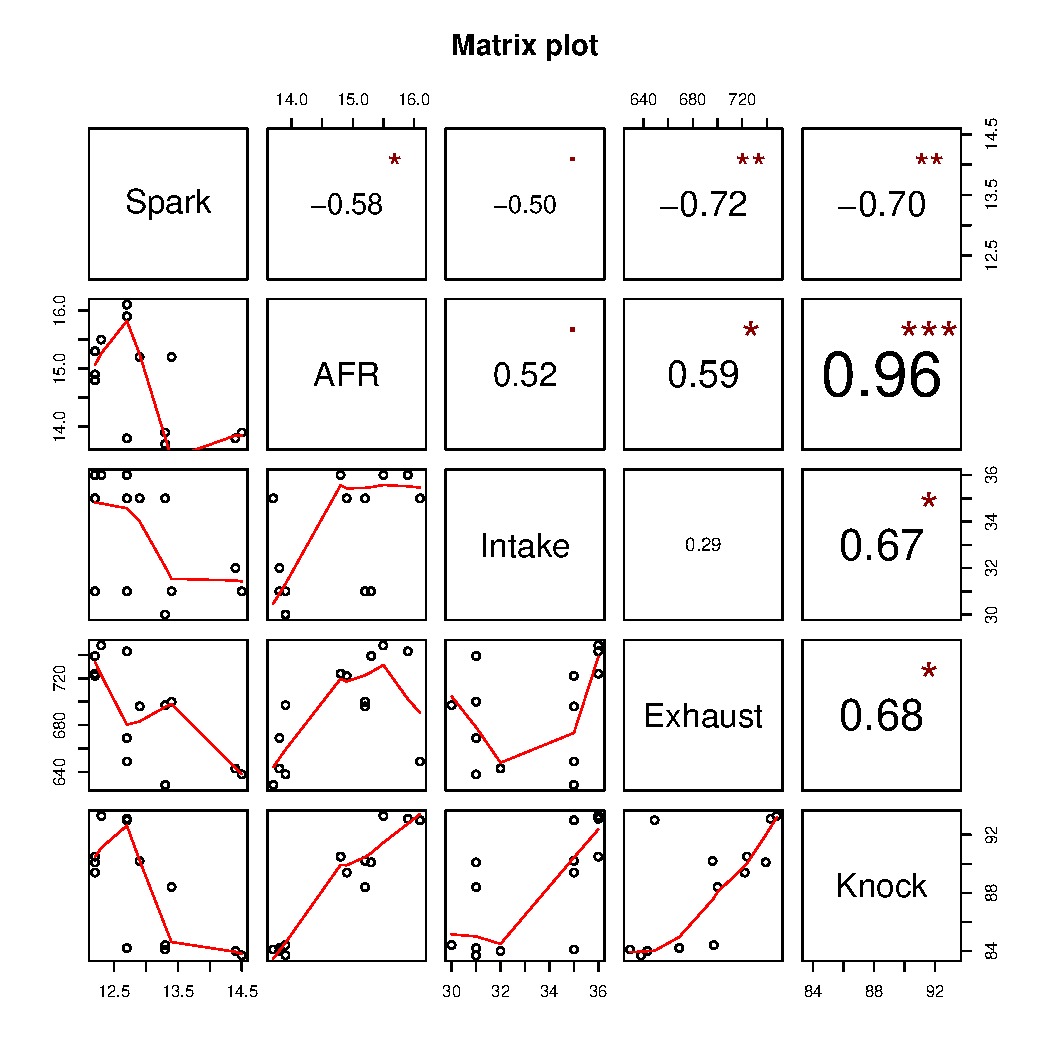
\includegraphics[width=7.5cm]{99_06_splmatKnock}
  \end{center}
\end{frame}

\begin{frame}
  \vspace{0.75cm}
  \begin{itemize}
    \item The graph shows each possible combination between the variables. The last line shows the scatterplot of \textit{Knock} and each of the predictors.
    \vspace{0.5cm}
    \item \textit{Knock} and \textit{Spark} seem to be negatively correlated; \textit{Knock} is positively correlated with each of other predictors.
  \end{itemize}
\end{frame}

\begin{frame}[fragile]
  Multiple regression analysis:\\
  \begin{small}
    \begin{verbatim}
Coefficients:
             Estimate Std. Error t value  p value    
(Intercept) 23.814922   8.136731   2.927  0.01909  
Spark       -0.296490   0.307181  -0.965  0.36271    
AFR          3.191814   0.239804  13.310  9.7e-07
Intake       0.358704   0.078482   4.571  0.00182
Exhaust      0.013376   0.005421   2.467  0.03886

Residual standard error: 0.5106 on 8 degrees of freedom
Multiple R-squared: 0.9879,	Adjusted R-squared: 0.9818 
F-statistic: 163.3 on 4 and 8 DF,  p-value: 1.062e-07
    \end{verbatim}
  \end{small}
  Anderson-Darling test:\\
  \begin{small}
    \begin{verbatim}
A = 0.3214, p-value = 0.4873
    \end{verbatim}
  \end{small}
\end{frame}

\begin{frame}
  \begin{small}
    \begin{itemize}
      \item The equation of the estimated regression model is: $ Knock = 23.8 - 0.296 \cdot Spark + 3.19 \cdot AFR + 0.359 \cdot Intake + 0.0134 \cdot Exhaust $
      \item The p-value of each variable specifies if It is significant in the current model. For example the variable \textit{Spark} seems to be not significant, but if we exclude the variable \textit{Exhaust} from the model, then \textit{Spark} becomes significant. This fact is due to the high correlation between the two variables.
      \item Overall the model explains the 98.79\% of the variability of the response; also the value of the adjusted $ R^2 $ (98.18\%) is very high.
      \item Then a step forward could be the estimation of a new regression model, without considering the variable \textit{Spark}, which is not significant.
      \item If more than a variable would not be significant, It is important deleting them one at a time.
    \end{itemize}
  \end{small}
\end{frame}

\begin{frame}[fragile]
  Multiple regression analysis:\\
  \begin{small}
    \begin{verbatim}
Coefficients:
             Estimate Std. Error t value  p value    
(Intercept) 16.487725   2.917508   5.651 0.000313
AFR          3.214814   0.237709  13.524 2.76e-07
Intake       0.386365   0.072784   5.308 0.000488
Exhaust      0.016576   0.004273   3.879 0.003737

Residual standard error: 0.5086 on 9 degrees of freedom
Multiple R-squared: 0.9865,	Adjusted R-squared: 0.982 
F-statistic: 219.1 on 3 and 9 DF,  p-value: 9.962e-09 
    \end{verbatim}
  \end{small}
  Anderson-Darling test:\\
  \begin{small}
    \begin{verbatim}
A = 0.1965, p-value = 0.8599
    \end{verbatim}
  \end{small}
\end{frame}

\begin{frame}
  \begin{small}
    \begin{itemize}
      \item The equation of the estimated regression model is: $ Knock = 16.5 + 3.21 \cdot AFR + 0.386 \cdot Intake + 0.0166 \cdot Exhaust $
      \item The $R^2$ of the model is clearly lower than that of the model with four predictors, and It is equal to 98.65\%.
      \item The adjusted $R^2$, on the other hand, is improved, and It is equal to 98.20\%.
      \item Because of also the graphics of the residuals (next slide) shows that all the assumptions about the errors have been satisfied, it is possible to consider this as a good model to explain the knocking engine.
    \end{itemize}
  \end{small}
\end{frame}

\begin{frame}
  Graphical check of the regression model multipla:\\
  \vspace{.1cm}
  \begin{center}
    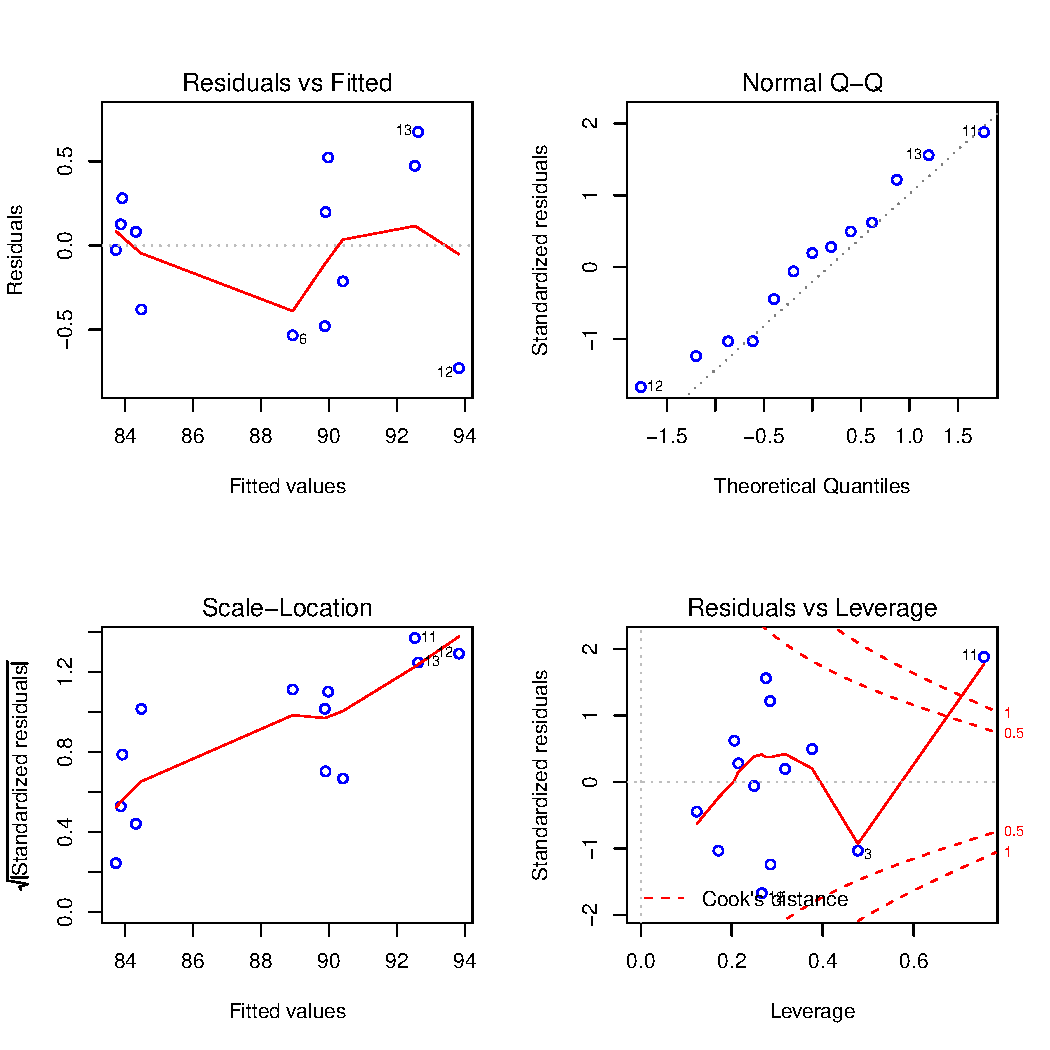
\includegraphics[width=7.5cm]{99_06_residPolKnock}
    \end{center}
\end{frame}

\livelloB{Mortality in the most important american cities}

\begin{frame}
  \begin{description}
    \item[Aims: ]
      \begin{footnotesize}
        The aim is to determine which variables are related with the percentage of mortality. Data was adapted from StatLib Website. 
        \begin{itemize}
          \item[-] Let us build the complete model, with all the regressors.
          \item[-] Let us reach to a model in which all the regressors have significant terms at the 5\% level, by eliminating a regressor at a time.
        \end{itemize}
      \end{footnotesize}
  \end{description}
\end{frame}

\begin{frame}
  \begin{description}
    \item[Data: ]mortality.txt \\ 
    \item[Description: ]
      \begin{footnotesize}
        \begin{itemize}
          \item \textit{Rain}: indicates the annual average rainfall;
          \item \textit{JanTemp}: indicates the average temperatures in January;
          \item \textit{JulyTemp}: indicates the average temperatures in July;
          \item \textit{PctOver65}: indicates the percentage of the population over 65 years;
          \item \textit{HHSize}: indicates the average size of housing;
          \item \textit{Education}: indicates the years of education;
          \item \textit{PctHomesLiveable}: indicates the percentage of ``habitable'' homes;
          \item \textit{PopDensity}: indicates the density of population;
          \item \textit{PctLowIncome}: indicates the percentage of low-income families;
          \item \textit{PctWhiteCollar}: indicates the percentage of employees;
          \item \textit{Hydrocarbon}: indicates the pollution level by hydrocarbons;
          \item \textit{NititeOxide}: indicates the pollution level of nitrite oxide;
          \item \textit{SulphurDioxide}: indicates the pollution level of sulfur dioxide;
          \item \textit{RelHum}: indicates the annual average relative humidity at 1 PM;
          \item \textit{MortalityRate}: indicates the mortality rate for 100'000 people.
        \end{itemize}
      \end{footnotesize}
  \end{description}
\end{frame}

\begin{frame}[fragile]
   Complete regression model:
  \begin{tiny}
    \begin{verbatim}
Coefficients:
                   Estimate Std. Error t value  p value    
(Intercept)       1.760e+03  4.270e+02   4.122 0.000159
Rain              1.916e+00  8.890e-01   2.156 0.036483
JanTemp          -1.976e+00  8.172e-01  -2.418 0.019714
JulyTemp         -3.115e+00  1.860e+00  -1.674 0.101021    
PctOver65        -9.218e+00  7.868e+00  -1.172 0.247501    
HHSize           -1.072e+02  6.862e+01  -1.562 0.125213    
Education        -1.714e+01  1.172e+01  -1.462 0.150678    
PctHomesLiveable -5.965e-01  1.404e+00  -0.425 0.673079    
PopDensity        3.625e-03  3.955e-03   0.917 0.364262    
PctLowIncome      4.424e+00  1.126e+00   3.930 0.000290
PctWhiteCollar   -1.704e-01  1.613e+00  -0.106 0.916322    
Hydrocarbon      -6.702e-01  4.841e-01  -1.385 0.173024    
NititeOxide       1.338e+00  9.935e-01   1.347 0.184813    
SulphurDioxide    8.686e-02  1.454e-01   0.597 0.553222    
RelHum            1.174e-01  1.139e+00   0.103 0.918323    

Residual standard error: 34.54 on 45 degrees of freedom
Multiple R-squared: 0.7649,	Adjusted R-squared: 0.6917 
F-statistic: 10.46 on 14 and 45 DF,  p-value: 6.576e-10 
    \end{verbatim}
  \end{tiny}
  Anderson-Darling test:\\
  \begin{small}
    \begin{verbatim}
A = 0.2774, p-value = 0.641
    \end{verbatim}
  \end{small}
\end{frame}

\begin{frame}
  \vspace{0.75cm}
  \begin{itemize}
    \item The complete model includes lots of non significant coefficients (at 5\% level).
    \vspace{0.75cm}
    \item Starting from the coefficient with the highest p-value, you must delete the non significant terms of the model one at a time. In this way, you arrive to the model displayed in the next slide.
    \vspace{0.75cm}
    \item Using other criterions to determine the significant variables, the resulting model could be different.
  \end{itemize}
\end{frame}

\begin{frame}[fragile]
  Reduced regression model:
  \begin{small}
    \begin{verbatim}
Coefficients:
              Estimate Std. Error t value  p value
(Intercept)  1145.1944    70.2397  16.304  < 2e-16
JanTemp        -1.5629     0.5937  -2.633  0.01103
Education     -19.3693     6.1794  -3.135  0.00278
PctLowIncome    4.4613     0.6531   6.831 7.75e-09
Hydrocarbon    -0.9844     0.3308  -2.976  0.00436
NititeOxide     1.9924     0.6341   3.142  0.00272

Residual standard error: 35.78 on 54 degrees of freedom
Multiple R-squared: 0.6972,	Adjusted R-squared: 0.6691 
F-statistic: 24.87 on 5 and 54 DF,  p-value: 6.603e-13 
    \end{verbatim}
  \end{small}
  \begin{small}
    Anderson-Darling test: \verb+A = 0.2651, p-value = 0.6824+
  \end{small}
\end{frame}

\begin{frame}
  Graphical check of the multiple regression model:\\
  \vspace{.1cm}
  \begin{center}
    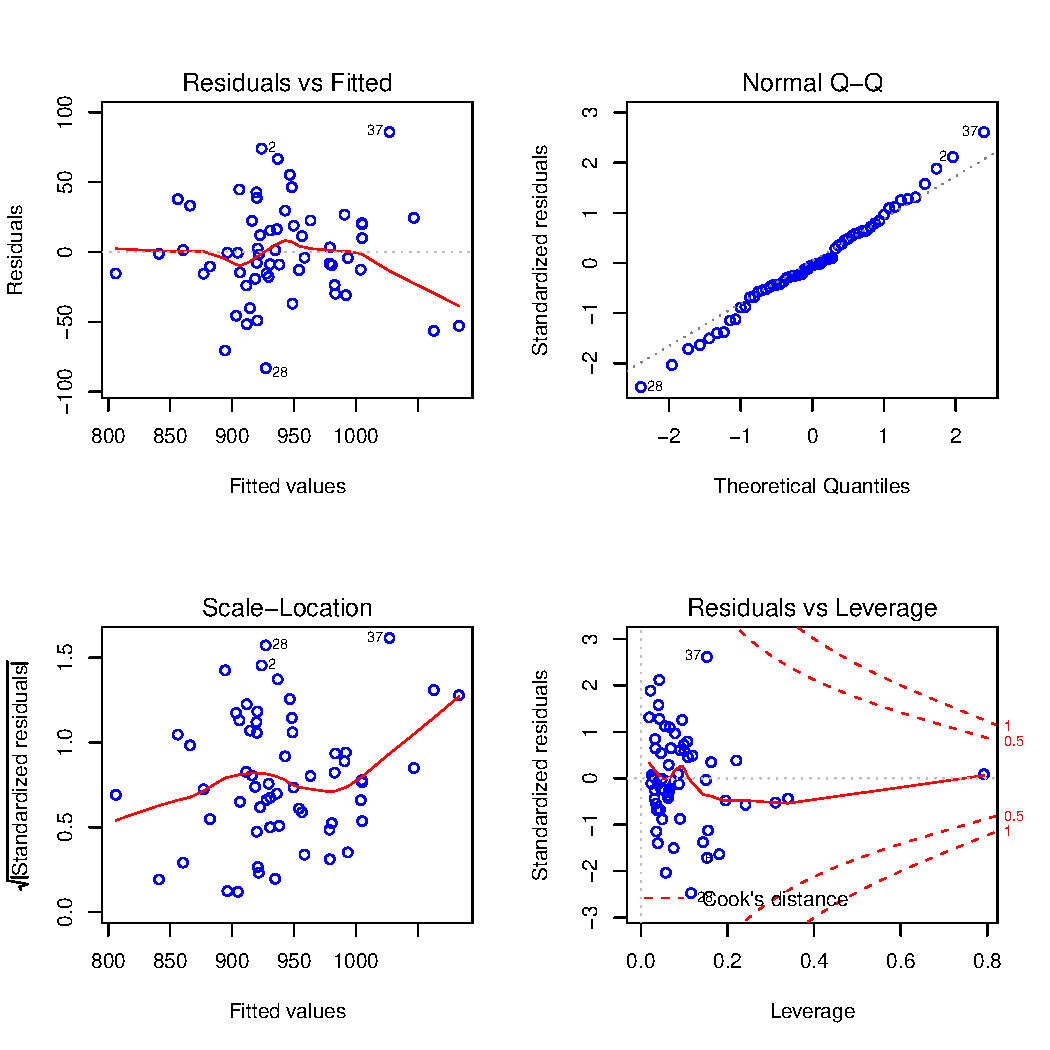
\includegraphics[width=7.5cm]{99_06_residPolMortalityRate}
  \end{center}
\end{frame}

\livelloB{Sleep duration}

\begin{frame}
  \begin{description}
    \item[Data: ]sleep.txt \\
    \item[Description: ]
      \begin{footnotesize}
        \begin{itemize}
          \item \textit{Species}: indicates the kind of animal (string);
          \item \textit{BodyWght}: indicates the weight (kg);
          \item \textit{MaxLife}: indicates the life duration (years);
          \item \textit{Gestation}: indicates the gestation period (days);
          \item \textit{Predation}: indicates the probability index for the animal to be preyed (from 1, lower probability, to 5);
          \item \textit{Exposure}: indicates the index of the level of exposure during sleep (from 1, animal who sleeps in a safe location, to 5);
          \item \textit{Sleep}: indicates the daily hours of sleep.
        \end{itemize}
      \end{footnotesize}
    \item[Aims: ]
      \begin{footnotesize}
        The aim is to determine which variable are related to the sleep duration in the 51 species analysed.
        \begin{itemize}
          \item[-] Let us build the complete model, with all the regressors.
          \item[-] Let us reach to a model in which all the regressors have significant terms at the 5\% level, by eliminating a regressor at a time.
        \end{itemize}
      \end{footnotesize}
  \end{description}
\end{frame}

\begin{frame}[fragile]
  Complete regression model:
  \begin{small}
    \begin{verbatim}
Coefficients:
              Estimate Std. Error t value  p value    
(Intercept) 16.9311593  1.1681738  14.494   <2e-16
BodyWght     0.0007099  0.0006693   1.061   0.2945    
MaxLife     -0.0181089  0.0342994  -0.528   0.6001    
Gestation   -0.0174520  0.0066645  -2.619   0.0120
Predation   -0.9063605  0.4593231  -1.973   0.0546
Exposure    -0.5386782  0.5294925  -1.017   0.3144 

Residual standard error: 3.234 on 45 degrees of freedom
Multiple R-squared: 0.5701,	Adjusted R-squared: 0.5223 
F-statistic: 11.94 on 5 and 45 DF,  p-value: 2.213e-07 
    \end{verbatim}
  \end{small}
  \vspace{-0.2cm}
  Anderson-Darling test: \verb+A = 0.5624, p-value = 0.1385+
\end{frame}

\begin{frame}
  \vspace{0.75cm}
  \begin{itemize}
\item The complete model includes lots of non significant coefficients (at 5\% level).
    \vspace{0.75cm}
    \item Starting from the coefficient with the highest p-value, you must delete the non significant terms of the model one at a time. In this way, you arrive to the model displayed in the next slide.
    \vspace{0.75cm}
    \item Using other criterions to determine the significant variables, the resulting model could be different.
  \end{itemize}
\end{frame}

\begin{frame}[fragile]
  Reduced regression model:
  \begin{small}
    \begin{verbatim}
Coefficients:
             Estimate Std. Error t value  p value   
(Intercept) 16.426357   1.045378  15.713  < 2e-16
Gestation   -0.018909   0.003259  -5.801 5.04e-07
Predation   -1.192701   0.311999  -3.823  0.00038

Residual standard error: 3.251 on 48 degrees of freedom
Multiple R-squared: 0.5367,	Adjusted R-squared: 0.5174 
F-statistic: 27.81 on 2 and 48 DF,  p-value: 9.54e-09 

    \end{verbatim}
  \end{small}
  \begin{small}
    Anderson-Darling test: \verb+A = 0.5876, p-value = 0.1192+
  \end{small}
\end{frame}

\begin{frame}
  Graphical check of the multiple regression model:\\
  \vspace{.1cm}
  \begin{center}
    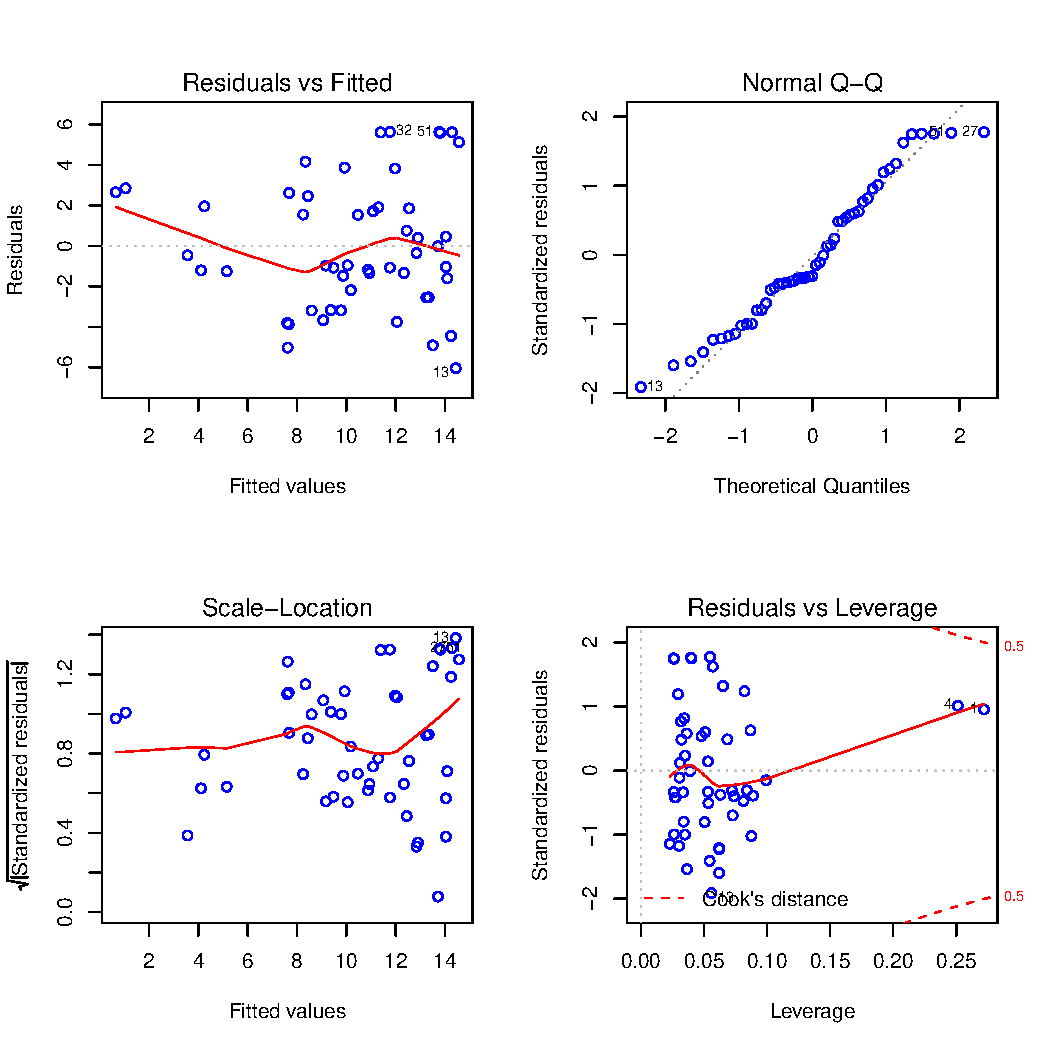
\includegraphics[width=7.5cm]{99_06_residPolSleep}
  \end{center}
\end{frame}



\livelloA{Regression with dummmy variables}

\livelloB{Weight differences between sexes}

\begin{frame}
  \begin{description}
    \item[Data: ]istat.txt \\ 
    \item[Description: ]
      \begin{footnotesize}
        \begin{itemize}
          \item \textit{Gender}: indicates the sex (factor);
          \item \textit{Area}: indicates the geographic area (factor);
          \item \textit{Weight}: indicates the weight (in kg);
          \item \textit{Height}: indicates the height (in cm).
        \end{itemize}
      \end{footnotesize}
      \begin{tiny}
        Data become to an ISTAT research of 2005 and interest the thirty-year-old italians.
      \end{tiny}
    \item[Aims: ]
      \begin{footnotesize}
        Let us study the differences in weight between the two sexes.
        \begin{itemize}
          \item[-] Use a t test for independent samples to check if there are differences in weight between male and female.  
          \item[-] Use, for the same check, a linear regression model.
        \end{itemize}
      \end{footnotesize}
  \end{description}
\end{frame}

\begin{frame}[fragile]
  \vspace{0.5cm}
  The t test for two independent samples gives the following result:
  \begin{small}
    \begin{verbatim}
t = -33.5243, df = 1804, p-value < 2.2e-16
alternative hypothesis: true difference in means
  is not equal to 0 
95 percent confidence interval:
 -17.26791 -15.35912 
    \end{verbatim}
  \end{small}
  It is necessary to note that the ``center'' of the 95\% level of the confidence interval for the real difference between means is  -16.31352 (point estimate). The reason will be clear in the next slide.
\end{frame}

\begin{frame}[fragile]
  A similar method to conduct the same comparison consists in using the linear regression model with an unique dummy variable as regressor, in addition to the intercept.
  \begin{small}
    \begin{verbatim}
Coefficients:
            Estimate Std. Error t value  p value   
(Intercept)  76.0668     0.3450  220.46   <2e-16
zFemale     -16.3135     0.4866  -33.52   <2e-16 

Residual standard error: 10.34 on 1804 degrees of freedom
Multiple R-squared: 0.3839,	Adjusted R-squared: 0.3835 
F-statistic:  1124 on 1 and 1804 DF,  p-value: < 2.2e-16 
    \end{verbatim}
  \end{small}
  Anderson-Darling test:\\
  \begin{small}
    \begin{verbatim}
A = 22.713, p-value < 2.2e-16
    \end{verbatim}
  \end{small}
\end{frame}

\begin{frame}
  \vspace{0.75cm}
  It is useful to note that:
  \begin{itemize}
    \vspace{0.5cm}
    \item The coefficient associated with the dummy variable has the same value of the point estimate of the difference between the means of the two groups;
    \vspace{0.5cm}
    \item The relative value of the index $ t $ is the same of the index $ t $ of the previous test.
  \end{itemize}
\end{frame}

\livelloB{Differences among sexes in the relationship between weight and height}

\begin{frame}
  \begin{description}
    \item[Data: ]istat.txt \\ 
    \item[Description: ]
      \begin{footnotesize}
        \begin{itemize}
          \item \textit{Gender}: indicates the sex (factor);
          \item \textit{Area}: indicates the geographic area (factor);
          \item \textit{Weight}: indicates the weight (in kg);
          \item \textit{Height}: indicates the height (in cm).
        \end{itemize}
      \end{footnotesize}
      \begin{tiny}
         Data become to an ISTAT research of 2005 and interest the thirty-year-old italians.
      \end{tiny}
    \item[Aims: ]
      \begin{footnotesize}
        The aim is to study if there are differences in the relation between weight and height due to sex.
       \begin{itemize}
          \item[-] Let us graphically represent the relation between weight and height, highlighting the different sex.
          \item[-] Let us compute a linear regression that considers the differences of intercept between male and female in the relation between weight and height.
          \item[-] Let us compute a linear regression that considers the differences of male and femal slope in the relation between weight and height.
          \item[-] Let us compute a linear regression that considers the differences both of intercept and of male and female slope in the relation between weight and height.
        \end{itemize}
      \end{footnotesize}
  \end{description}
\end{frame}

\begin{frame}
  \vspace{-0.3cm}
  \begin{center}
    \includegraphics[scale=0.45]{99_06_regrDummy1}
  \end{center}
\end{frame}

\begin{frame}[fragile]
  Regression analysis with dummy variables\\ (difference of intercept) :\\
  \begin{small}
    \begin{verbatim}
Coefficients:
             Estimate Std. Error t value  p value   
(Intercept) -39.23019    5.99508  -6.544  7.8e-11
x             0.65415    0.03397  19.258  < 2e-16
zFemale      -8.71260    0.59353 -14.679  < 2e-16

Residual standard error: 9.419 on 1803 degrees of freedom
Multiple R-squared: 0.489,	Adjusted R-squared: 0.4884 
F-statistic: 862.6 on 2 and 1803 DF,  p-value: < 2.2e-16 
    \end{verbatim}
  \end{small}
  Anderson-Darling test:\\
  \begin{small}
    \begin{verbatim}
A = 27.0344, p-value < 2.2e-1
    \end{verbatim}
  \end{small}
\end{frame}

\begin{frame}
  \vspace{0.5cm}
  \begin{itemize}
    \item The equation of the estimated regression model is: $ Weight = -39.23 + 0.654 \cdot Height - 8.713 \cdot Female $
    \item If the subject is male, then \textit{Female} is equal to 0 and so the model equation becomes: $ Weight = -39.23 + 0.654 \cdot Height $; if the subject is female, the model equation becomes  $ Weight = -47.94 + 0.654 \cdot Height $
    \item The dummy coefficient related to the difference of intercept between sexes is significant.
    \item $R^2$ of the model is equal to 48.90\%.
    \item The graphic is the next slide shows the two estimated regression lines.
  \end{itemize}
\end{frame}

\begin{frame}
  \vspace{-0.3cm}
  \begin{center}
    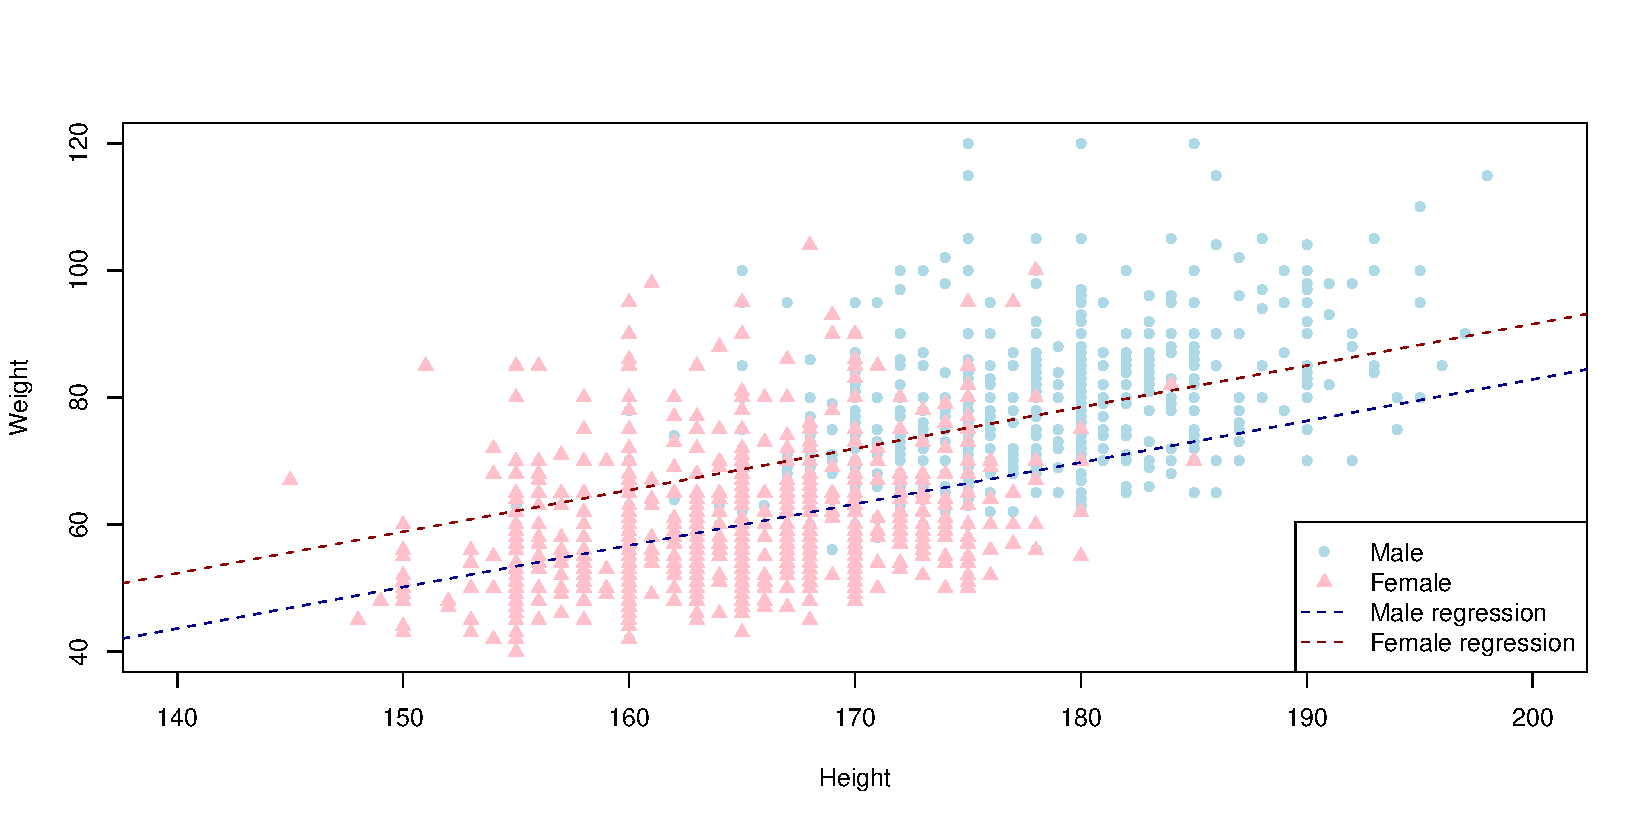
\includegraphics[scale=0.45]{99_06_regrDummy2}
  \end{center}
\end{frame}

\begin{frame}[fragile]
  Regression analysis with dummy variables\\ (difference of slope):\\
  \begin{small}
    \begin{verbatim}
Coefficients:
              Estimate Std. Error t value  p value   
(Intercept) -42.333280   5.792810  -7.308 4.06e-13
x             0.671981   0.032864  20.447  < 2e-16
x:zFemale    -0.052143   0.003483 -14.970  < 2e-16

Residual standard error: 9.399 on 1803 degrees of freedom
Multiple R-squared: 0.4911,	Adjusted R-squared: 0.4906 
F-statistic: 870.1 on 2 and 1803 DF,  p-value: < 2.2e-16 
    \end{verbatim}
  \end{small}
  Anderson-Darling test:\\
  \begin{small}
    \begin{verbatim}
A = 27.3062, p-value < 2.2e-16
    \end{verbatim}
  \end{small}
\end{frame}

\begin{frame}
  \begin{small}
    \begin{itemize}
      \item The equation of the estimated regression model is: $ Weight = -42.33 + 0.672 \cdot Height - 0.052 \cdot Height \cdot Female $
      \item If the subject is a male, than \textit{Female} is equal to 0 and so the equation of the model becomes: $ Weight = -42.33 + 0.672 \cdot Height $; if the subject is a female then the equation becomes $ Weight = -42.33 + 0.667 \cdot Height $
      \item The coefficient of the dummy variable related to the difference of slope among sexes is significant.
      \item The $R^2$ of the model is 49.11\%.
      \item The graphics of the next slides shows the two estimated regression lines. The first graph shows the graph starting from the origin of axes. In this way It is clear that the two lines have the same intercept. The second graph shows only the part of plan that includes the points. This part is highlighted by a black box in the first graph.  
    \end{itemize}
  \end{small}
\end{frame}

\begin{frame}
  \vspace{-0.3cm}
  \begin{center}
    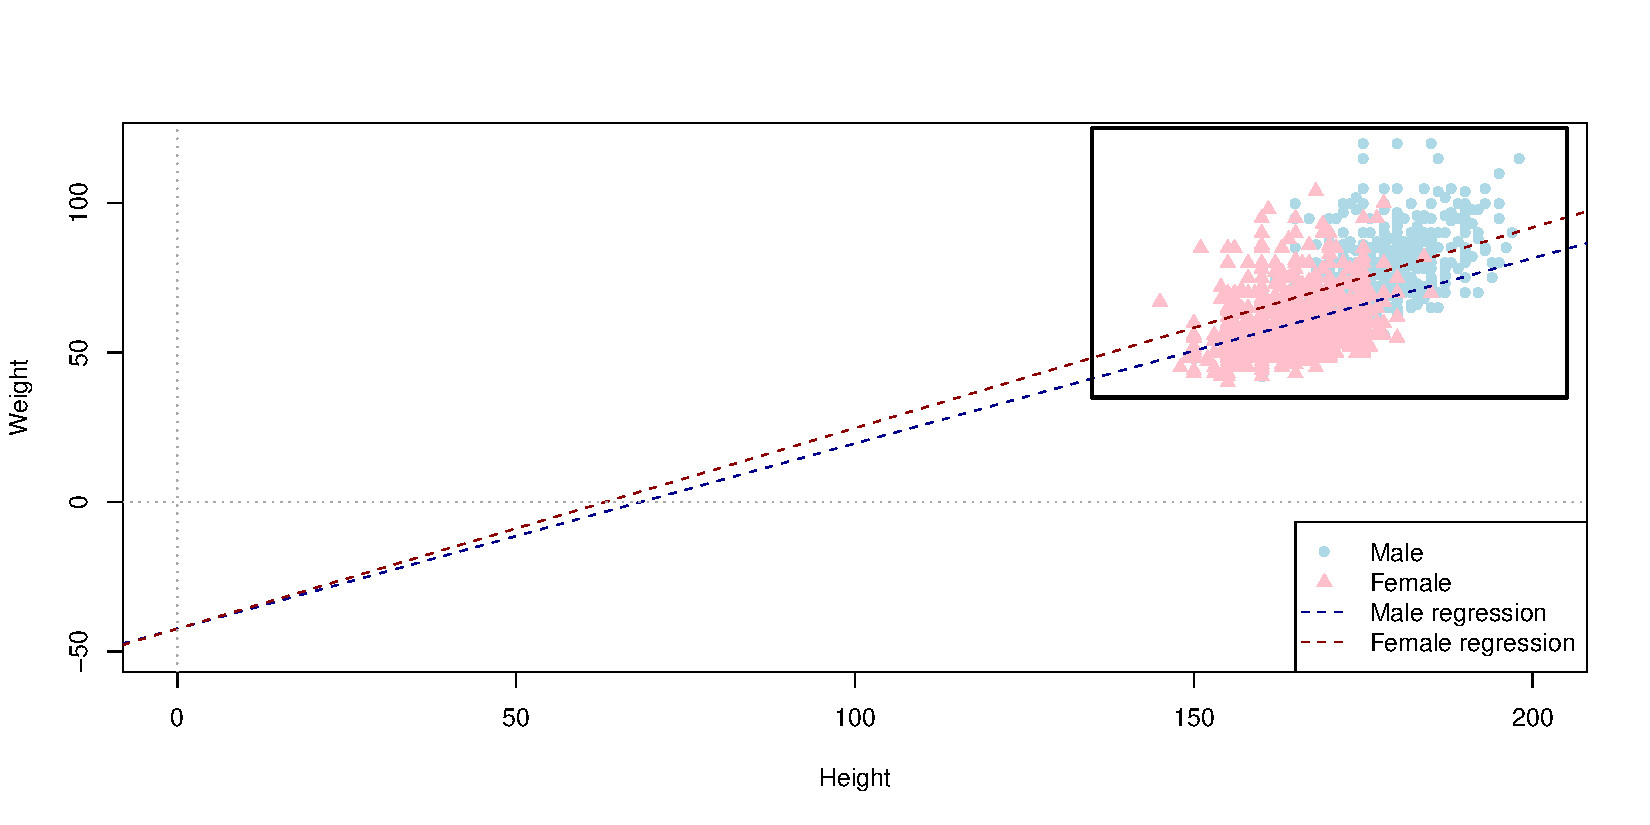
\includegraphics[scale=0.45]{99_06_regrDummyCA1}
  \end{center}
\end{frame}

\begin{frame}
  \vspace{-0.3cm}
  \begin{center}
    \includegraphics[scale=0.45]{99_06_regrDummyCA2}
  \end{center}
\end{frame}

\begin{frame}[fragile]
  Regression analysis with dummy variables\\ (differences both of intercept and of slope):\\
  \begin{small}
    \begin{verbatim}
Coefficients:
             Estimate Std. Error t value  p value    
(Intercept) -68.44263    7.98282  -8.574  < 2e-16
x             0.81989    0.04526  18.116  < 2e-16
zFemale      54.44344   11.52739   4.723 2.50e-06
x:zFemale    -0.37191    0.06779  -5.486 4.70e-08

Residual standard error: 9.344 on 1802 degrees of freedom
Multiple R-squared: 0.4974,	Adjusted R-squared: 0.4965 
F-statistic: 594.4 on 3 and 1802 DF,  p-value: < 2.2e-16 
    \end{verbatim}
  \end{small}  
  Anderson-Darling test:\\
  \begin{small}
    \begin{verbatim}
A = 26.6082, p-value < 2.2e-16
    \end{verbatim}
  \end{small}
\end{frame}

\begin{frame}
  \vspace{0.5cm}
  \begin{itemize}
    \item The equation of the estimated model is: $ Weight = -68.44 + 0.820 \cdot Height - 54.44 \cdot Female - 0.372 \cdot Height \cdot Female $
    \vspace{0.15cm}
    \item If the subject is a male, than \textit{Female} is equal to 0 and so the equation of the model is: $ Weight = -68.44 + 0.820 \cdot Height $; if the subject is a female than the eqaution becomes $ Weight = -14.00 + 0.44798 \cdot Height $
    \vspace{0.15cm}
    \item The coefficients are all significant.
    \vspace{0.15cm}
    \item $R^2$ of the model is 49.74\%.
    \vspace{0.15cm}
    \item The graph in the next slide shows the two estimated regression lines.
  \end{itemize}
\end{frame}

\begin{frame}
  \vspace{-0.3cm}
  \begin{center}
    \includegraphics[scale=0.45]{99_06_regrDummyAll1}
  \end{center}
\end{frame}


\livelloB{Differences among geographical areas in the relation between weight and height}

\begin{frame}
  \begin{description}
    \item[Data: ]istat.txt \\ 
    \item[Description: ]
      \begin{footnotesize}
        \begin{itemize}
          \item \textit{Gender}: indicates the sex (factor);
          \item \textit{Area}: indicates the geographic area (factor);
          \item \textit{Weight}: indicates the weight (in kg);
          \item \textit{Height}: indicates the height (in cm).
        \end{itemize}
      \end{footnotesize}
      \begin{tiny}
       Data become to an ISTAT research of 2005 and interest the thirty-year-old italians.
      \end{tiny}
    \item[Aims: ]
      \begin{footnotesize}
        The aim is to study if in the relation between weight and height there are differences due to the geographical area of residence (North, Centre, South and Islands).
       \begin{itemize}
          \item[-] Let us graphically represent the relation between weight and heigh, highlighting the different geographical areas.
          \item[-] Let us compute a linear regression that considers the differences of intercept among the different geographical areas in the relation between weight and height.
        \end{itemize}
      \end{footnotesize}
  \end{description}
\end{frame}

\begin{frame}
  \vspace{-0.3cm}
  \begin{center}
    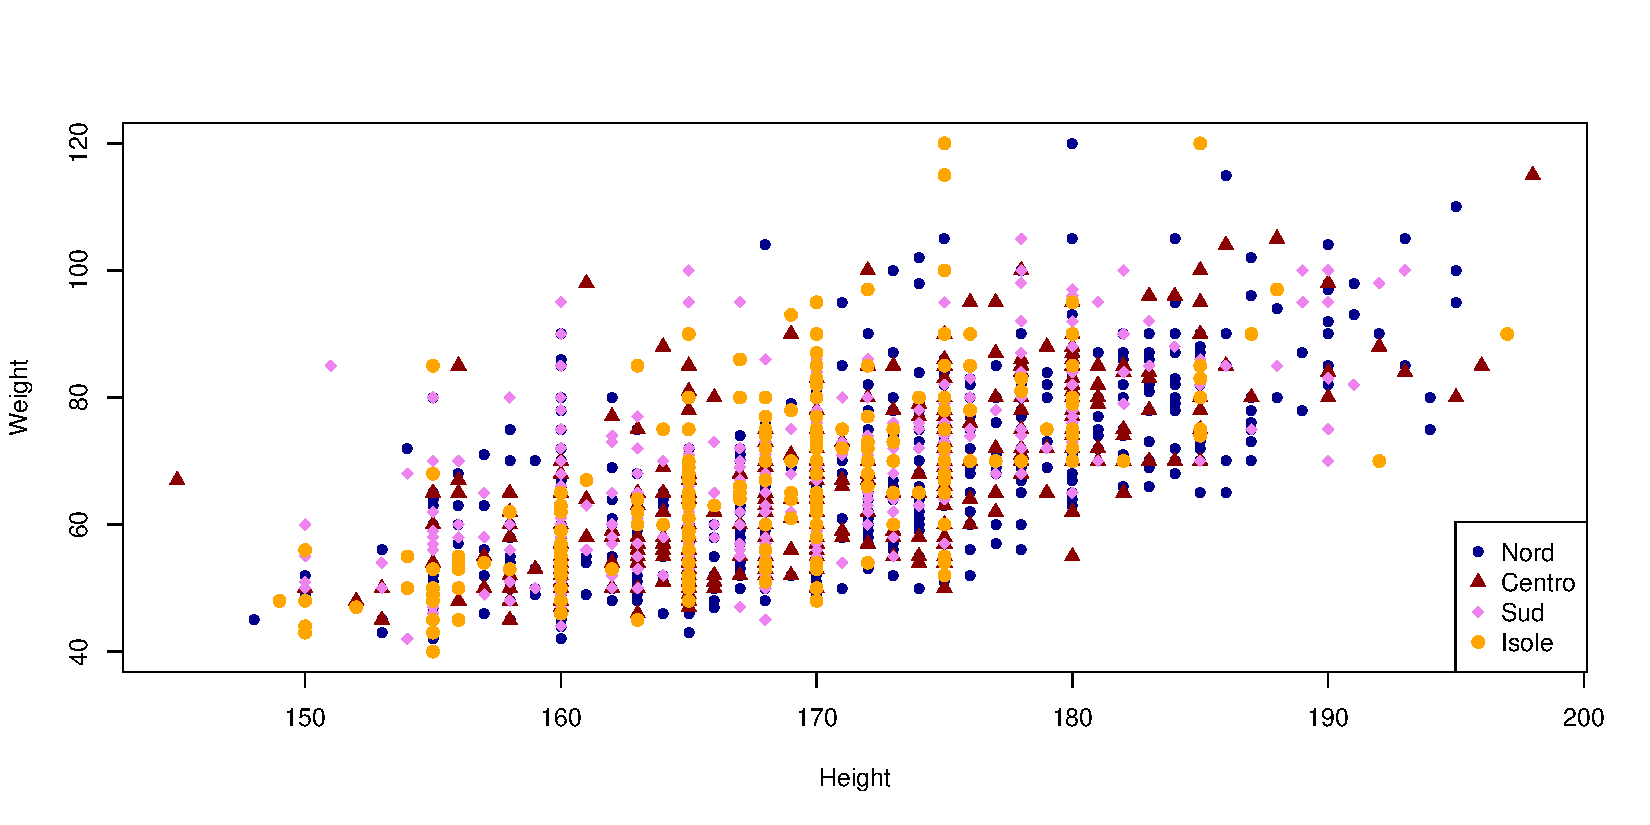
\includegraphics[scale=0.45]{99_06_regrDummy3}
  \end{center}
\end{frame}

\begin{frame}[fragile]
  Regression analysis with dummy variables\\ (differences of intercept):\\
  \begin{small}
    \begin{verbatim}
Coefficients:
              Estimate Std. Error t value  p value    
(Intercept) -104.37815    4.60721 -22.655  < 2e-16
x              1.00532    0.02679  37.521  < 2e-16
zIsole         2.70906    0.84250   3.216  0.00133 
zNord         -0.25560    0.61924  -0.413  0.67983    
zSud           2.74037    0.68021   4.029 5.84e-05

Residual standard error: 9.873 on 1801 degrees of freedom
Multiple R-squared: 0.4392,	Adjusted R-squared: 0.4379 
F-statistic: 352.6 on 4 and 1801 DF,  p-value: < 2.2e-16 
    \end{verbatim}
  \vspace{-0.5cm}
  Anderson-Darling test: \verb+A = 14.1561, p-value < 2.2e-16+
  \end{small}
\end{frame}

\begin{frame}
  \vspace{0.5cm}
  \begin{itemize}
    \item The geographical area ``Centre'' represents the baseline, or reference. The coefficients relative to the others geographical areas represent the deviation of the intercept from the coefficient of the region Centre.
    \vspace{0.25cm}
    \item For $ \alpha = 0.05 $, the coefficient of South and Islands are significant.
    \vspace{0.25cm}
    \item $R^2$ of the model is 43.92\%.
    \vspace{0.25cm}
    \item The graph in the next slide shows the estimated regression lines. It is possible to note as the estimated regression lines of North and Centre are closer each other; in the same way those relative to the South and the Islands.
  \end{itemize}
\end{frame}

\begin{frame}
  \vspace{-0.3cm}
  \begin{center}
    \includegraphics[scale=0.45]{99_06_regrDummy4}
  \end{center}
\end{frame}

\begin{frame}[fragile]
  Regression analysis with dummy variables\\ (differences both of intercept and of slope):\\
  \begin{small}
    \begin{verbatim}
Coefficients:
              Estimate Std. Error t value Pr(>|t|)    
(Intercept) -1.032e+02  9.950e+00 -10.370   <2e-16
zIsole      -1.651e+01  1.662e+01  -0.994    0.321    
zNord       -1.410e+00  1.212e+01  -0.116    0.907    
zSud         9.432e+00  1.373e+01   0.687    0.492    
x            9.983e-01  5.813e-02  17.172   <2e-16
zIsole:x     1.138e-01  9.788e-02   1.162    0.245    
zNord:x      6.753e-03  7.075e-02   0.095    0.924    
zSud:x      -3.963e-02  8.063e-02  -0.492    0.623

Residual standard error: 9.874 on 1798 degrees of freedom
Multiple R-squared:  0.44,	Adjusted R-squared: 0.4378 
F-statistic: 201.8 on 7 and 1798 DF,  p-value: < 2.2e-16 
    \end{verbatim}
  \end{small}
\end{frame}

\begin{frame}
  \vspace{0.5cm}
  \begin{itemize}
    \item The previous slide shows the regression analysis with differences both of intercept and of slope.
    \vspace{0.25cm}
    \item For $ \alpha = 0.05 $, none coefficient of the dummy variables seems to be significant.
    \vspace{0.25cm}
    \item It is not correct to eliminate all the non significant terms: we must always eliminate one at a time.
    \vspace{0.25cm}
    \item At the end of a backwise procedure, the resulting model is the same displayed previously. The difference is only the intercept.
  \end{itemize}
\end{frame}



\livelloA{Linearizable models}

\livelloB{Body weight and brain weight}

\begin{frame}
  \begin{description}
    \item[Data: ]brainbod.txt \\ 
    \item[Description: ]
      \begin{footnotesize}
        \begin{itemize}
          \item \textit{Species}: indicates the animal species (string);
          \item \textit{Body}: indicates the weight of the animal (in kg);
          \item \textit{Brain}: indicates the weight of the brain of the animal (in g).
        \end{itemize}
      \end{footnotesize}
    \item[Aims: ]
      \begin{footnotesize}
        The aim is to establish if there is a relation between the weight of the body and the weight of the brain of fifteen mammal (african elephant, cow, monkey, man, gray wolf, red fox, armadillo, chinchilla and so on).
        \begin{itemize}
          \item[-] Let us show the descriptive univariate graphics (histograms and BW plot) of the two variables.
          \item[-] Let us show a scatterplot of the two variables and let us estimate a linear regression model.       
          \item[-] The linear model between the two variables is adequate? Why? How could it been improved?
        \end{itemize}
      \end{footnotesize}
  \end{description}
\end{frame}

\begin{frame}
  Descriptive graphics:\\
  \vspace{-0.3cm}
  \begin{center}
    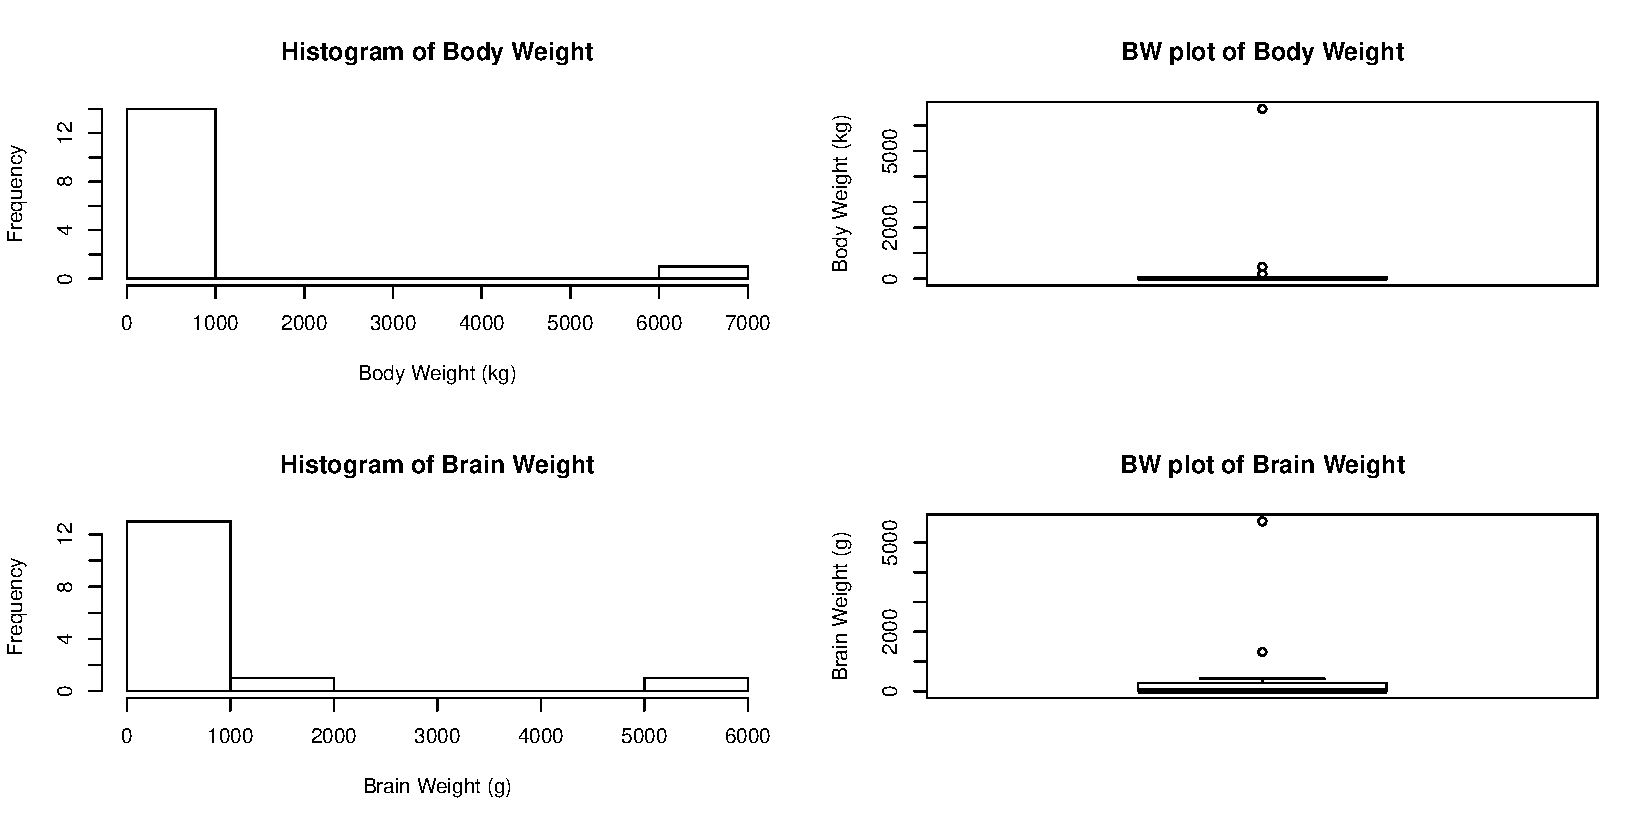
\includegraphics[scale=0.45]{99_06_modLin1}
  \end{center}
\end{frame}

\begin{frame}
  \vspace{0.5cm}
  Scatterplot:\\
  \vspace{-0.8cm}
  \begin{center}
    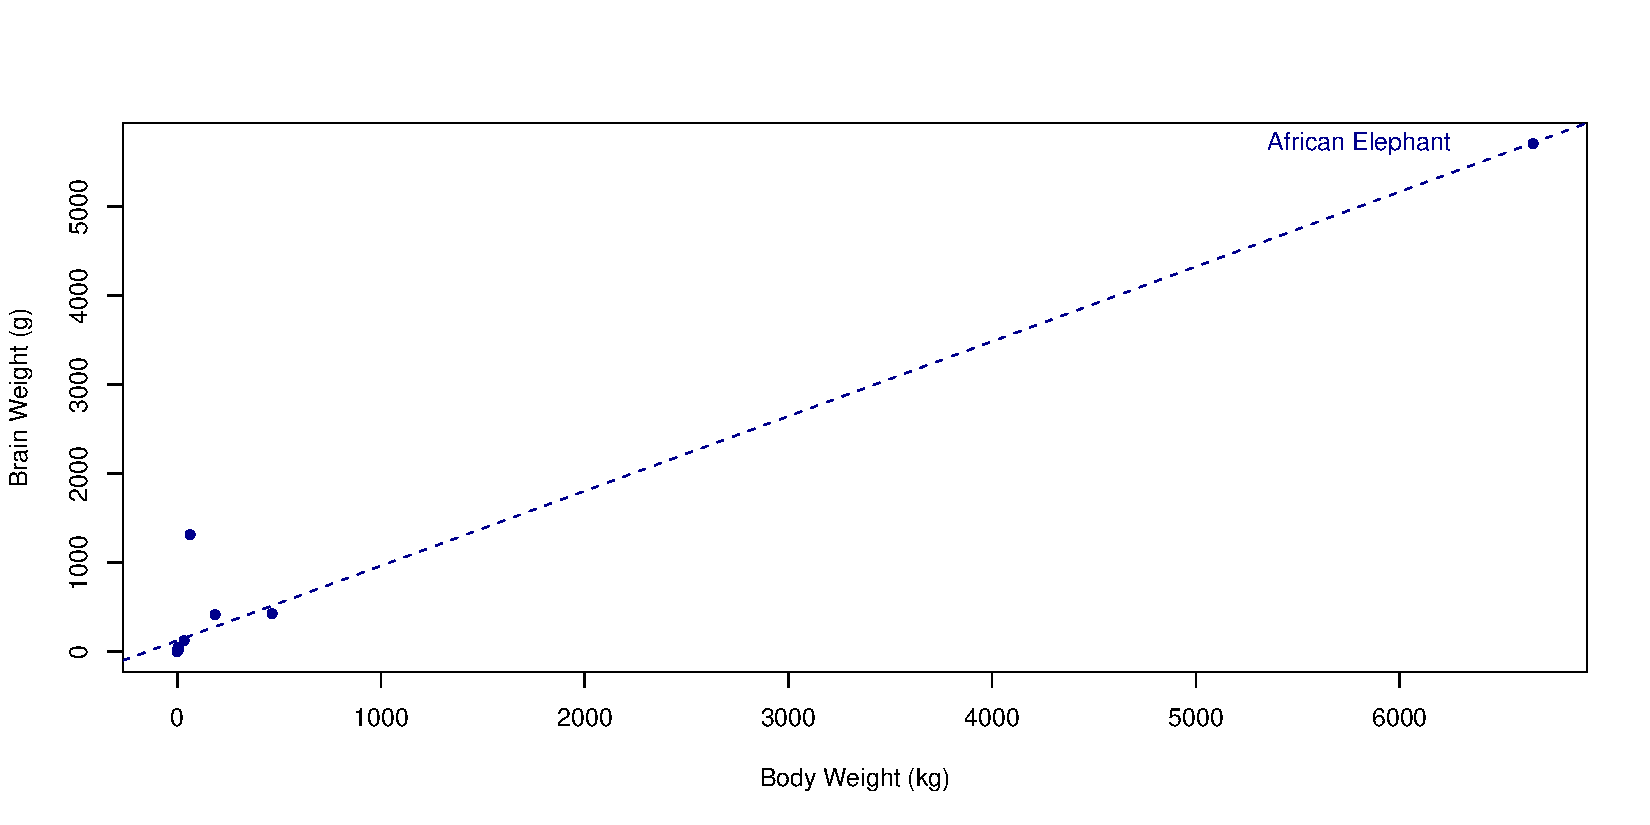
\includegraphics[scale=0.45]{99_06_modLin2}
  \end{center}
\end{frame}

\begin{frame}[fragile]
  Regression analysis:\\
  \begin{small}
    \begin{verbatim}
Coefficients:
             Estimate Std. Error t value  p value    
(Intercept) 124.52517   90.60557   1.374    0.193    
x             0.84086    0.05259  15.990 6.26e-10

Residual standard error: 336.1 on 13 degrees of freedom
Multiple R-squared: 0.9516,	Adjusted R-squared: 0.9479 
F-statistic: 255.7 on 1 and 13 DF,  p-value: 6.257e-10 
    \end{verbatim}
  \end{small}
  Anderson-Darling test:\\
  \begin{small}
    \begin{verbatim}
A = 3.5975, p-value = 1.677e-09
    \end{verbatim}
  \end{small}
\end{frame}

\begin{frame}
  Graphical check of the regression model:\\
  \vspace{.1cm}
  \begin{center}
    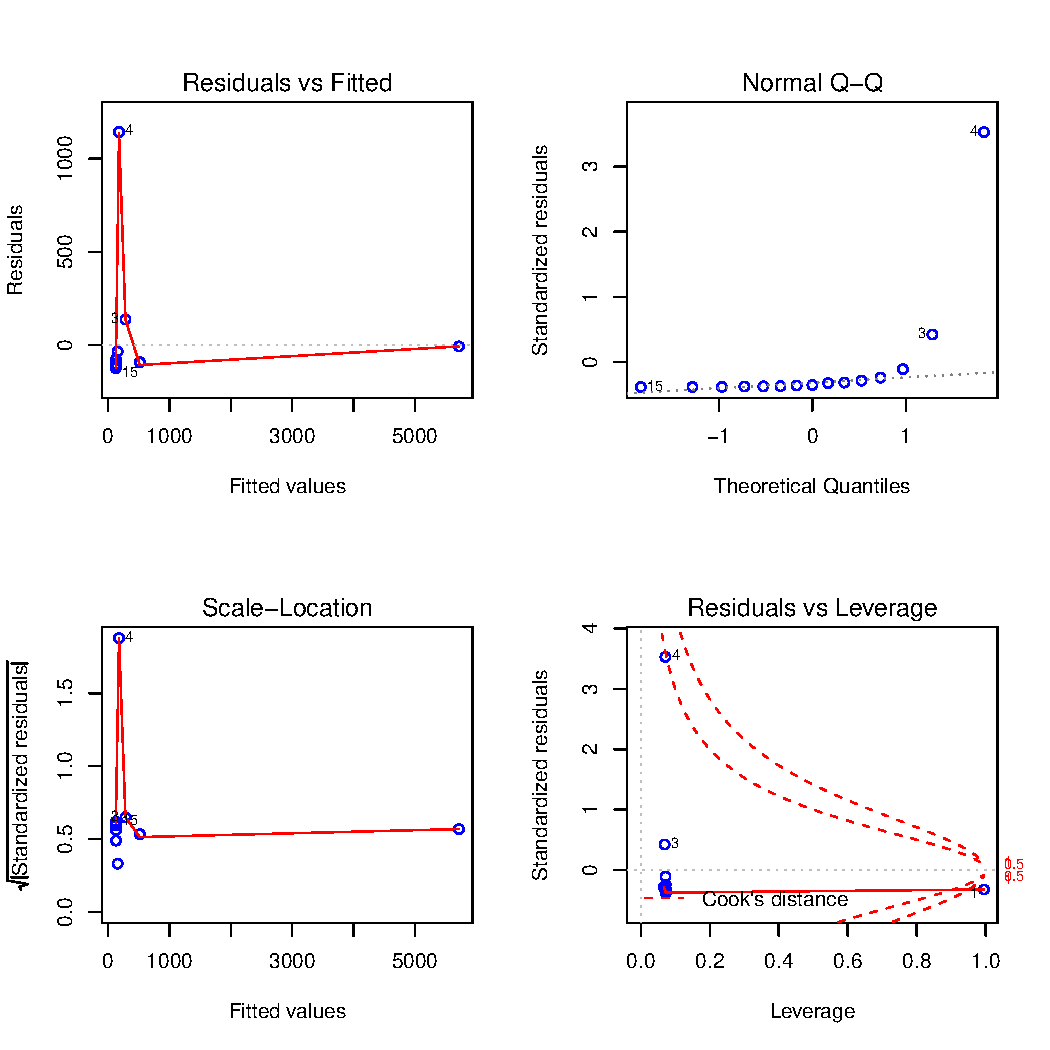
\includegraphics[width=7.5cm]{99_06_resid1SetPoint}
    \end{center}
\end{frame}

\begin{frame}
  \vspace{0.5cm}
  \begin{itemize}
    \item A linear regression seems to exist between the two variables.
    \vspace{0.35cm}
    \item An high value of the$ R^2 $ (95.16\%) implies that the link between body weight and brain weight is well explained by a linear regression.
    \vspace{0.35cm}
    \item However, the weight of the African elephant is much higher than that of other animals, and It makes the graph and the regression curve illegible.
    \vspace{0.35cm}
    \item A logarithmic transformation of the two variables may suggest a more clear reading of the graph and It may show understandably the relation between the two variables.
  \end{itemize}
\end{frame}

\begin{frame}
  descriptive graphics:\\
  \vspace{-0.3cm}
  \begin{center}
    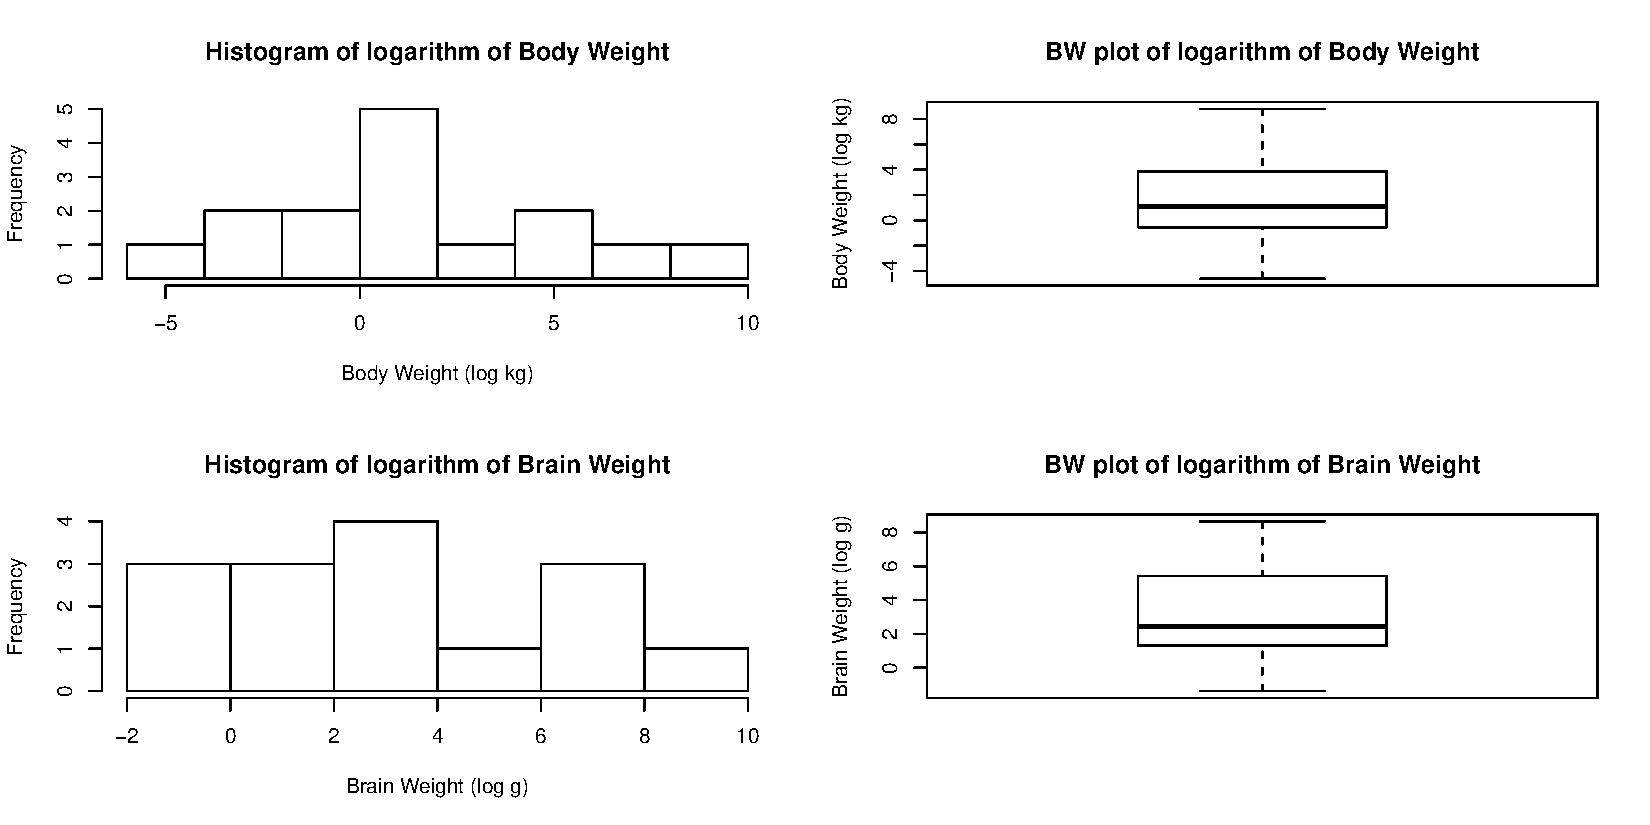
\includegraphics[scale=0.45]{99_06_modLin3}
  \end{center}
\end{frame}

\begin{frame}
  \vspace{0.5cm}
  Scatterplot:\\
  \vspace{-0.8cm}
  \begin{center}
    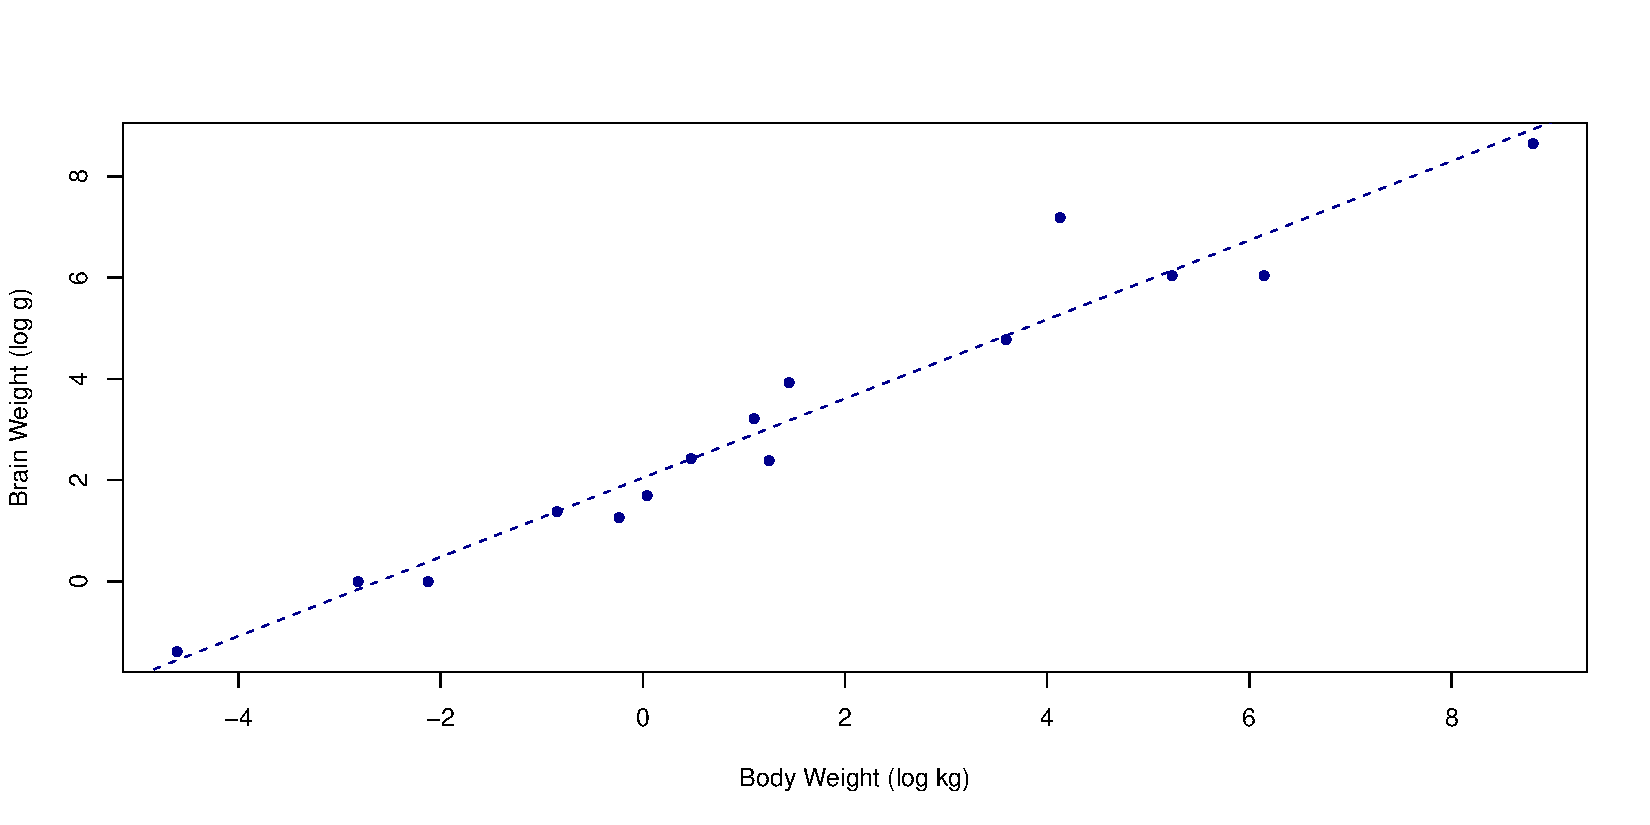
\includegraphics[scale=0.45]{99_06_modLin4}
  \end{center}
\end{frame}

\begin{frame}[fragile]
  Regression analysis:\\
  \begin{small}
    \begin{verbatim}
Coefficients:
            Estimate Std. Error t value  p value    
(Intercept)  2.04818    0.19261   10.63 8.78e-08
log(x)       0.78218    0.05123   15.27 1.11e-09

Residual standard error: 0.6891 on 13 degrees of freedom
Multiple R-squared: 0.9472,	Adjusted R-squared: 0.9431 
F-statistic: 233.1 on 1 and 13 DF,  p-value: 1.110e-09  
    \end{verbatim}
  \end{small}
  Anderson-Darling test:\\
  \begin{small}
    \begin{verbatim}
A = 0.7164, p-value = 0.04826
    \end{verbatim}
  \end{small}
\end{frame}

\begin{frame}
  Graphical check of the regression model:\\
  \vspace{.1cm}
  \begin{center}
    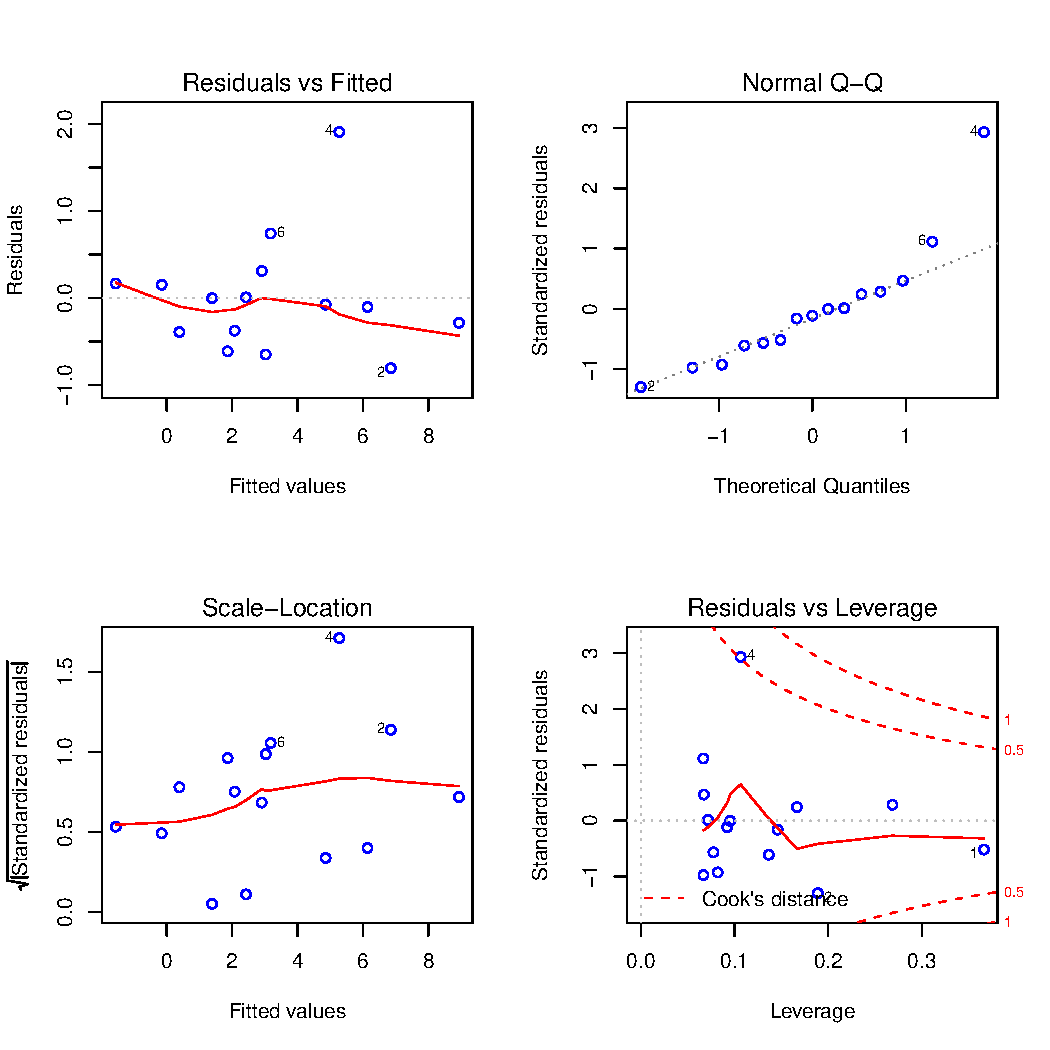
\includegraphics[width=7.5cm]{99_06_resid2SetPoint}
    \end{center}
\end{frame}

\begin{frame}
  \vspace{0.75cm}
  \begin{itemize}
    \item The scatterplot of the logarithms of the weights seems to be more clear than in the same graph on the original data. 
.
    \vspace{0.5cm}
    \item Moreover, the Anderson-Darling test rejects the hypothesis of residual normality, for all values of $\alpha$ among those commonly used. However, in the model that considers logarithmic transformation the hypothesis of residual normality seems to be accepted.
  \end{itemize}
\end{frame}



\livelloA{Forecasting}

\livelloB{Impurities in paints}

\begin{frame}
  \begin{description}
    \item[Data: ]paint.txt \\ 
    \item[Description: ]
      \begin{footnotesize}
        \begin{itemize}
         \item \textit{Stirrate}: identifies the rate of agitation (revolution) applied to the container (rpm, revolutions per minute);
          \item \textit{Impurity}: indentifies the number of impurities (lumps) present in the containers of paint.
        \end{itemize}
      \end{footnotesize}
    \item[Aims: ]
      \begin{footnotesize}
        The number of impurities (lumps) present in the containers of paint depends on the rate of agitation applied to the container. Previously we determined the linear relation that links the revolution rate applied to the container with the number of lumps. We want to use that relation to forecast the number of lumps present in the container with varinish, starting from the applied agitation rate.
        \begin{itemize}
          \item[-]  Let us estimate the value of \textit{Impurity} if \textit{Stirrate} is equal to 30.
          \item[-]  Let us estimate the confidence and prediction intervals at 95 \% level for the linear regression model.
          \item[-]  Let us estimate a prediction interval of \textit{Impurity} at 95 \% level if \textit{Stirrate} is equal to 30.
        \end{itemize}
      \end{footnotesize}
  \end{description}
\end{frame}

\begin{frame}
  Scatterplot of the relation with regression line:\\
  \vspace{.3cm}
  \begin{center}
    \includegraphics[width=7.5cm]{99_06_regrPred30StirrateImpurity.pdf}
  \end{center}
\end{frame}

\begin{frame}
  Regression line with confidence and prediction intervals at 95\% level:\\
  \vspace{.3cm}
  \begin{center}
    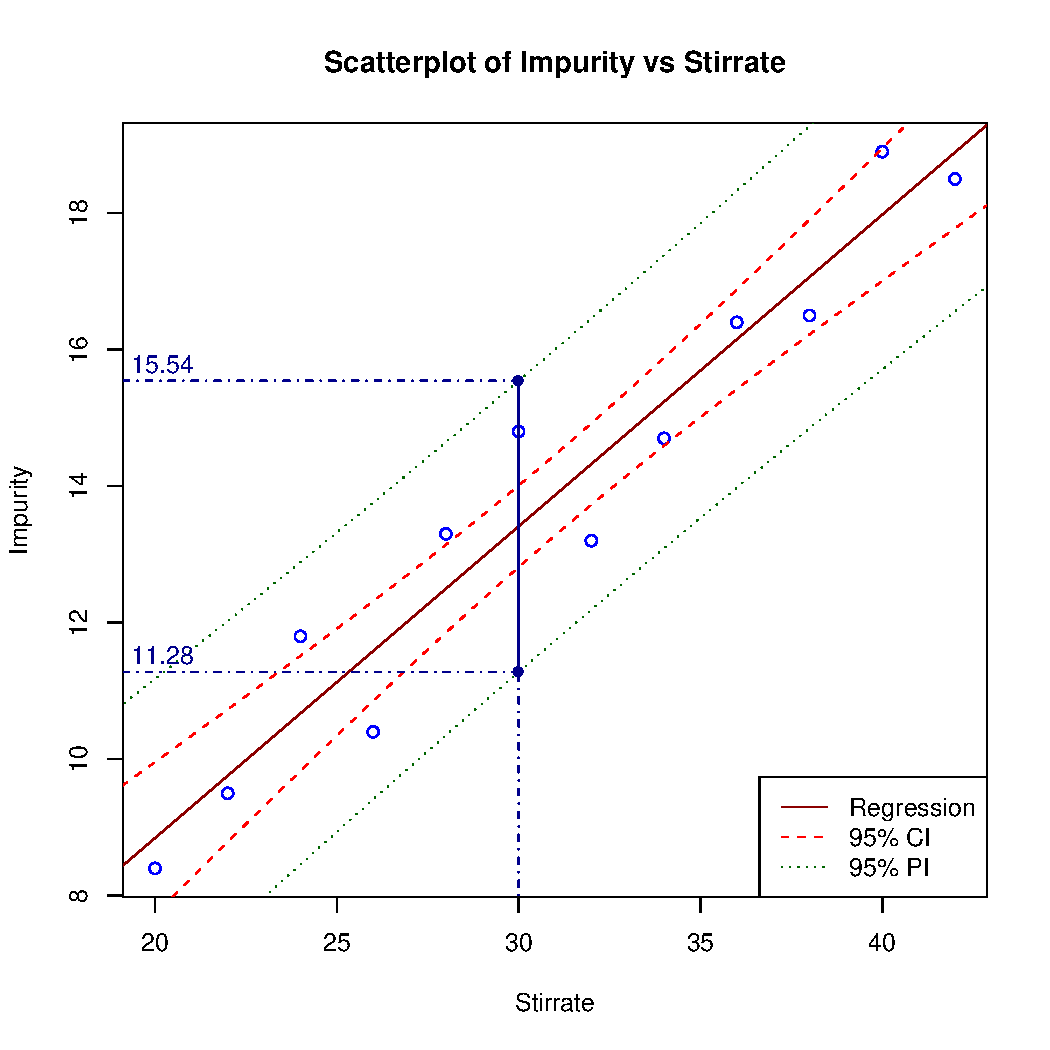
\includegraphics[width=7.5cm]{99_06_regrInt30StirrateImpurity.pdf}
  \end{center}
\end{frame}

\begin{frame}
  \vspace{.25cm}
  \begin{small}
  \begin{itemize}
     \item A possible use of the linear regression model to make predictions on \textit{Stirrate} values not present in the sample.
     \item For example, let us assume you want to estimate the number of impurities present in the containers of paint when the revolution rate is equal to 30 rpm.
     \item The first graph shows than an estimate (punctual) of the number of impurities is 13.41. It means that you can expect about 13 impurities.
     \item It is necessary to consider the variability of the estimates of the model, so the prediction interval, built starting from the regression line, must be used.
     \item Let us assume a value of \textit{Stirrate} equal to 30, the 95\% level prediction interval is 11.28 - 15.54. It means that the number of lumps can vary from 11 to 16, when the revolutio rate is equal to 30 rpm. 
  \end{itemize}
  \end{small}
\end{frame}



\livelloA{Covariance analysis}

\livelloB{Effect of susceptibility to hypnosis}

\begin{frame}
  \begin{description}
    \item[Data: ]suggestibility.txt \\ 
    \item[Description: ]
      \begin{footnotesize}
        \begin{itemize}
          \item \textit{Induction}: indicates the score of the induction to hypnosis (from 1 to 50);
          \item \textit{Suggestibility}: indicates the score of punteggio di susceptibility (from 1 to 50);
          \item \textit{Method}: indicates the type of medicine (factor).
        \end{itemize}
      \end{footnotesize}
    \item[Aims: ]
      \begin{footnotesize}
        The aim is to establish if two hypnotic medicines, A and B, are equally effective in inducing the hypnotic state in patients. However, the effective of the hypnotic induction is subjective because It depends on the individual susceptibility of the patient. Then, before the medicine administration, the subjects have to do a susceptibility test to hypnosis.
        \begin{itemize}
          \item[-] Let us show, at least graphically, that the differences between the two medicines, A e B, are much more evident when the component due to the susceptibility of the patient is removed.
        \end{itemize}
      \end{footnotesize}
  \end{description}
\end{frame}

\begin{frame}
  \vspace{0.5cm}
  The following slide shows three graphics that highlight how:
  \begin{itemize}
    \vspace{0.25cm}
    \item without considering the individual susceptibility of the patients, the induction to hypnosis is similar between subjects treated with medicine A and those treated with medicine B, as the left graph shows;
    \vspace{0.25cm}
    \item the susceptibility and the induction to hypnosis is different in the two groups, as the central graph shows;
    \vspace{0.25cm}
    \item in fact, when you removed the component due to susceptibility, the induction to hypnosis of the subjects treated with medicine A is greater than the induction to hypnosis of the subjects treated with medicine B, as the right graph shows.
  \end{itemize}
\end{frame}

\begin{frame}
  \vspace{-0.3cm}
  \begin{center}
    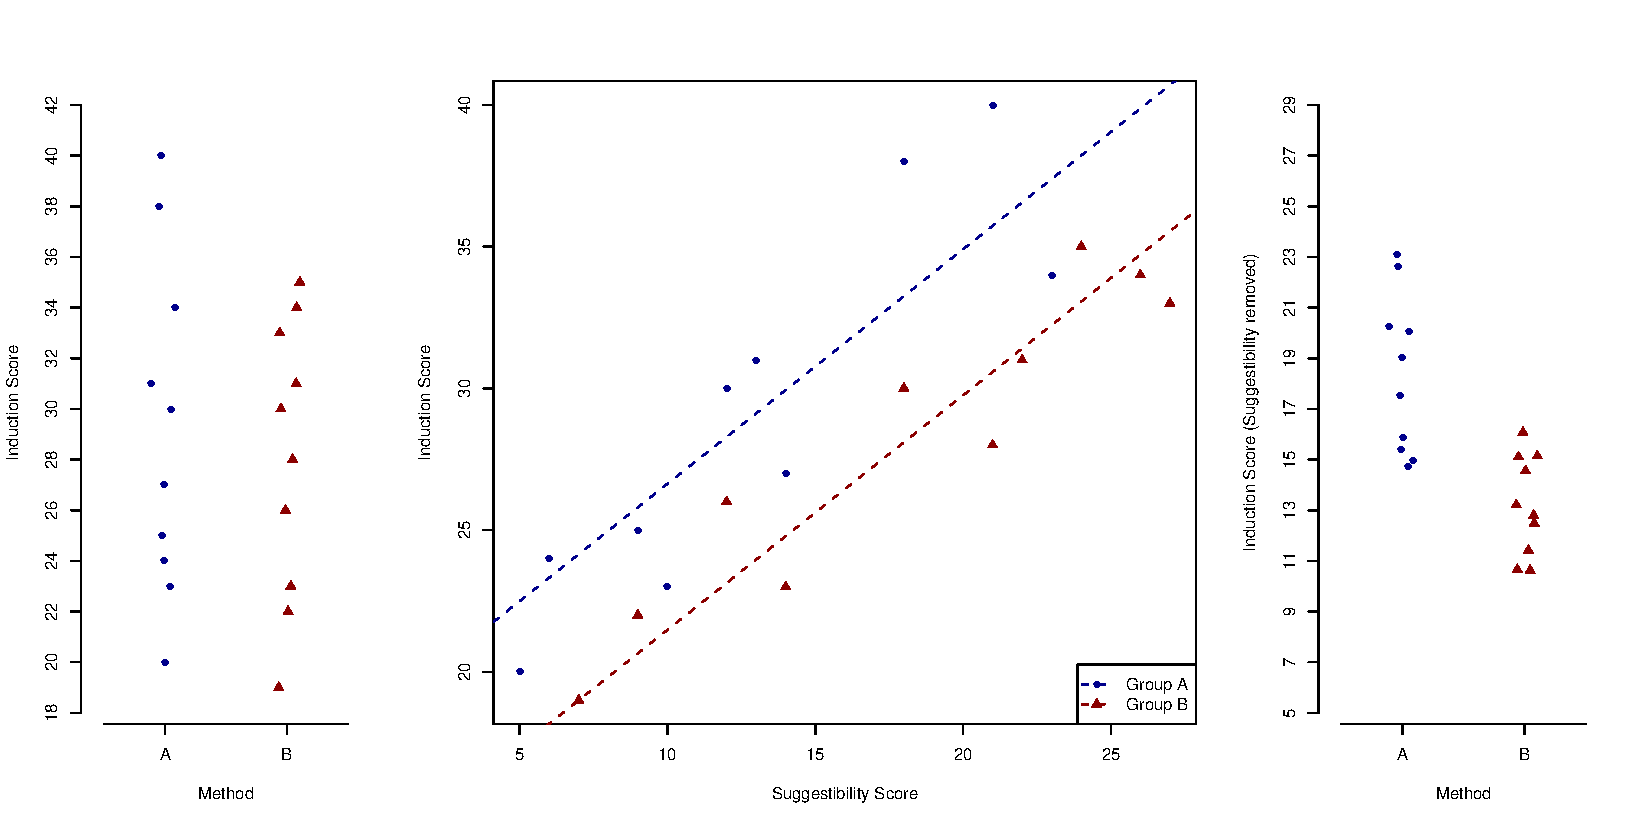
\includegraphics[scale=0.45]{99_06_ancova1}
  \end{center}
\end{frame}

\livelloB{Effect of the height on the obesity}

\begin{frame}
  \begin{description}
    \item[Data: ]weight.txt \\ 
    \item[Description: ]
      \begin{footnotesize}
        \begin{itemize}
          \item \textit{Region}: indicates the region of residence (factor);
          \item \textit{Weight}: indicates the weight (in kg);
          \item \textit{Height}: indicates the height (in cm).
        \end{itemize}
      \end{footnotesize}
    \item[Aims: ]
      \begin{footnotesize}
        The aim is to establish if the inhabitants of two italian regions close to each other, Lombardy and Veneto, have different ``obesity''. 
        The weight is used as obesity index.
        \begin{itemize}
          \item[-] Let us show how, at least graphically, the differences between the ``obesity'' of the Lombardy and Veneto inhabitants are due to the different heights of the subjects of both groups.
        \end{itemize}
      \end{footnotesize}
  \end{description}
\end{frame}

\begin{frame}
  \vspace{0.5cm}
  The following slide shows three graphs that highlight how:
  \begin{itemize}
    \vspace{0.25cm}
    \item the obesity, without considering the height, is lower for Veneto inhabitants, as the left graph shows;
    \vspace{0.25cm}
    \item the weight and height are different in the two regions, as the central graph shows;
    \vspace{0.25cm}
    \item in fact, when you removed the component due to the differences in height, the degree of obesity of the Veneto inhabitants not seem to be different from that of the Lombardy inhabitants.
  \end{itemize}
\end{frame}

\begin{frame}
  \vspace{-0.3cm}
  \begin{center}
    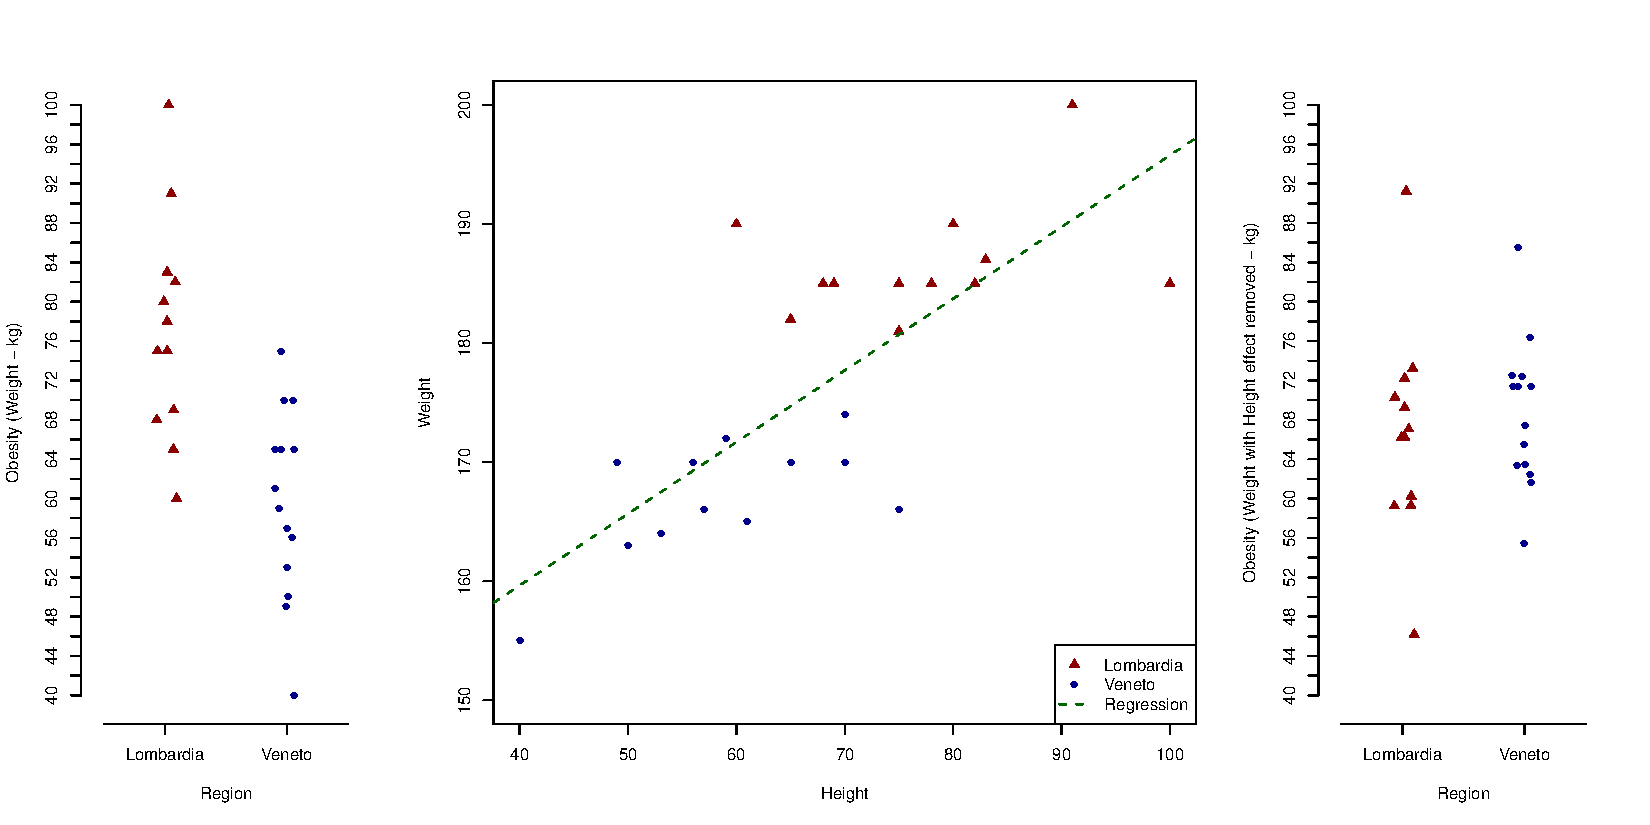
\includegraphics[scale=0.45]{99_06_ancova2}
  \end{center}
\end{frame}



